\chapter{信息量}
\label{chap:information-measures}

一个结果按概率$\tfrac12,\tfrac14,\tfrac18,\tfrac18$出现在四个字母$a,b,c,d$中。朋友知道结果，我们只能问是非题。先问“是$a$吗”，有一半机会一题就猜中；否则再问“是$b$吗”，依此类推，平均要问$1.75$题。若四个字母等可能，平均就要问$2$题。分布越集中，平均要问的题越少。能不能用一个只依赖概率表的数，衡量一个随机结果平均含有多少不确定性？

再看两个相关的结果。一枚公平硬币$X$经过一条会以概率$\tfrac14$出错的线路，收到的是$Y$。看到$Y$以后，$X$并没有被完全确定，但比看到之前清楚了一些。清楚了多少？如果再把$Y$经过同样的线路传一次，或者把$Y$压缩成更粗的摘要，能不能反而更清楚？如果要从$Y$猜出$X$，错误概率最低能低到哪里？

本章研究这些问题。第一节从单个结果的意外程度出发，定义自信息与熵，先在离散情形建立它的基本性质，再说明对密度计算的微分熵改变了什么。第二、三节研究两个变量：联合熵与条件熵度量整体和剩余的不确定性，互信息度量观测带来的不确定性的减少，并用联合分布与边缘乘积的KL散度给出不依赖熵是否有限的一般定义。第四节讨论按一个参考分布分配对数代价时多付的部分，即交叉熵。

后四节用这些量研究信息处理的限制。数据处理不等式说明对观测作任何只依赖观测本身的处理都不能增加信息；Fano不等式把剩余的不确定性转成辨别错误的下界；在互信息难以直接计算时，用辨认真配对的辅助问题可以得到它的一个可计算的下界；最后讨论信息量随分布连续变化需要什么条件。

全章以自然对数为准，信息量的单位是nat；需要以“题数”或二进制位数解释时换成以$2$为底的对数，单位是bit。两个贯穿的小例子是上面的四字母表和公平硬币经过出错线路的二元表，后面还会用到一张不对称的$2\times2$联合表。怎样用最少的码字实际描述结果、怎样在有噪声的线路上可靠地传输，分别在第~\ref{chap:lossless-coding}章和第~\ref{chap:discrete-channel-capacity}章研究；本章只建立这些任务所用的量及其界。

\section{熵}
\label{sec:info-entropy}

天气预报说明天有雨，在雨季几乎不值得一提，在旱季却是大新闻。同一句话带来的信息多少，取决于它事先有多意外。本节先给单个结果的意外程度一个数值，再对所有可能结果取平均，得到衡量随机结果不确定性的熵。离散结果可以直接这样做；对有密度的连续结果照搬公式时，会多出一个依赖坐标尺度的量，需要单独说明。

\subsection{自信息}
\label{sec:info-self-information}

设某个结果发生的概率是$p\in(0,1]$。我们想给它指定一个数$c(p)$，表示“得知这个结果发生”所获得的信息量。至少有两个要求是自然的。

第一，越罕见的结果越意外，信息越多，所以$c$是$(0,1]$上的递减函数；必然发生的结果不带来信息，$c(1)=0$。第二，两个独立结果同时发生的概率是$pq$，分别得知它们和一起得知它们，获得的信息应当一样多，所以
\[
  c(pq)=c(p)+c(q),\qquad 0<p,q\leq1.
\]
回到章首的四字母表：结果$c$的概率是$\tfrac18$，它相当于连续三次“二选一”都选中某一边，每次概率$\tfrac12$；按第二个要求，它的信息量应是$\tfrac12$对应信息量的三倍。

\begin{theorem}[自信息的形式]
\label{thm:info-self-information-form}
设$c:(0,1]\to[0,\infty)$递减且对一切$p,q\in(0,1]$满足$c(pq)=c(p)+c(q)$，则存在常数$a\geq0$，使
\begin{equation}
  c(p)=-a\ln p,\qquad 0<p\leq1.
  \label{eq:info-self-information-form}
\end{equation}
\end{theorem}

\begin{proof}
令$b(u)=c(\mathrm{e}^{-u})$，$u\geq0$。指数函数把加法变成乘法，所以$c$的乘法关系变成$b$的加法关系：
\[
  b(u+v)=b(u)+b(v),\qquad u,v\geq0.
\]
$u$增大时$\mathrm{e}^{-u}$减小，$c$递减，所以$b$在$[0,\infty)$上递增。

先看有理点。由可加性，$b(0)=b(0)+b(0)$，故$b(0)=0$；对正整数$n$，$b(nu)=nb(u)$。取$u=1/m$，得$b(1)=m\,b(1/m)$，于是对正整数$n,m$，
\[
  b\Bigl(\frac{n}{m}\Bigr)=n\,b\Bigl(\frac1m\Bigr)=\frac{n}{m}\,b(1).
\]
记$a=b(1)\geq b(0)=0$，则$b(r)=ar$对一切非负有理数$r$成立。

再看一般的$u\geq0$。对任意有理数$r\leq u\leq s$，单调性给出$ar=b(r)\leq b(u)\leq b(s)=as$。让$r,s$从两侧趋于$u$，得$b(u)=au$。代回$u=-\ln p$，即得式~\eqref{eq:info-self-information-form}。
\end{proof}

证明里两个要求各起一个作用：可加性把$c$在有理点上的值全部确定下来，单调性把有理点之间的空隙填满。只有可加性而没有任何正则性时，满足$b(u+v)=b(u)+b(v)$的函数可以极不规则，结论就不再成立。常数$a$不受这两个要求约束，它只决定信息量的单位。

\begin{definition}[自信息]
\label{def:info-self-information}
设离散随机变量$X$的概率质量为$p_X$。对$p_X(x)>0$的取值$x$，称
\begin{equation}
  \iota(x)=-\ln p_X(x)
  \label{eq:info-self-information}
\end{equation}
为结果$x$的\term{自信息}（self-information），单位为\term{奈特}（nat）。若改用$-\log_2 p_X(x)$，单位为\term{比特}（bit）。
\end{definition}

两种单位只差一个正的常数倍：$-\log_2 p=-\ln p/\ln2$，所以
\[
  1\ \mathrm{bit}=\ln2\ \mathrm{nat}\approx0.693\ \mathrm{nat}.
\]
换单位不改变任何两个信息量的大小顺序，也不改变“相等”“为零”这类结论。本章用nat计算，以bit解释“是非题个数”。

比特的说法来自是非题。一个概率为$2^{-k}$的结果，自信息是$k$ bit，恰好相当于连续回答$k$个各占一半的是非题。图~\ref{fig:info-self-information}画出$-\ln p$，右侧刻度换成bit。$p$从$1$减小到$\tfrac12$只带来$1$ bit，而每再减半一次就多$1$ bit；概率趋于零时自信息趋于无穷。

\begin{BookInlineFigure}
  \centering
  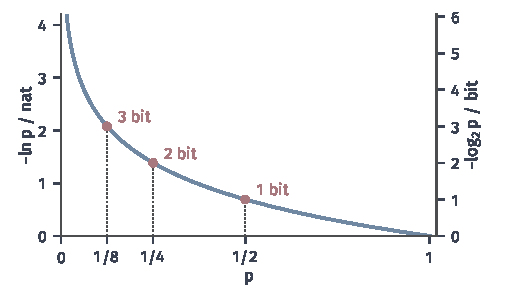
\includegraphics[width=86mm]{figures/07-probability/04-distribution-analysis/matplotlib/info-self-information/figure.pdf}
  \caption{自信息随概率的变化。蓝线为$-\ln p$，左轴以nat计，右轴为同一曲线以bit计的刻度。红点是四字母表中概率$\tfrac12,\tfrac14,\tfrac18$的结果，分别对应$1,2,3$ bit。}
  \label{fig:info-self-information}
\end{BookInlineFigure}

自信息是一次结果的属性。看到罕见结果时获得很多信息，但罕见结果很少出现；要衡量一个随机结果“平均”含有多少信息，还要按概率取平均。

\subsection{离散熵}
\label{sec:info-discrete-entropy}

章首的四字母表可以按图~\ref{fig:info-question-tree}的方式提问。每个结果所需的题数恰好是它以bit计的自信息：$a$一题，$b$两题，$c,d$各三题。平均题数是
\[
  \tfrac12\cdot1+\tfrac14\cdot2+\tfrac18\cdot3+\tfrac18\cdot3=1.75.
\]
这就是自信息的平均。对一般的概率表，题数必须是整数，不一定能与自信息一一相等；第~\ref{chap:lossless-coding}章证明，最好的提问方案平均题数与以bit计的熵相差不到一题。

\begin{BookInlineFigure}
  \centering
  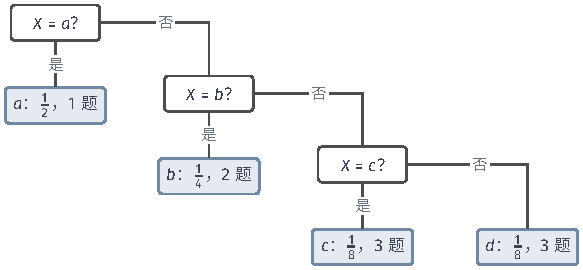
\includegraphics[width=98.7mm]{figures/07-probability/04-distribution-analysis/tikz/info-question-tree/figure.pdf}
  \caption{四字母表$(\tfrac12,\tfrac14,\tfrac18,\tfrac18)$的一种是非题提问方案。蓝框是确定下来的结果，框内为其概率与所需题数；每个结果的题数等于$-\log_2 p$，平均题数为$1.75$。}
  \label{fig:info-question-tree}
\end{BookInlineFigure}

\begin{definition}[离散熵]
\label{def:info-discrete-entropy}
设离散随机变量$X$取值于有限或可数集合$\mathcal{X}$，概率质量为$p_X$。$X$的\term{熵}（entropy）定义为
\begin{equation}
  H(X)=-\sum_{x\in\mathcal{X}}p_X(x)\ln p_X(x)=\mathbb{E}[-\ln p_X(X)],
  \label{eq:info-entropy}
\end{equation}
其中约定$0\ln0=0$。各项非负，和可以为$+\infty$。
\end{definition}

约定$0\ln0=0$有两个理由。概率为零的结果从不出现，不应影响平均；并且$t\ln t\to0$（$t\downarrow0$），约定与极限一致，加入或删去零概率的取值都不改变熵。熵只依赖概率值的集合，与取值叫什么无关：把$a,b,c,d$换成$1,2,3,4$或任意排列，熵不变。这一点与期望、方差不同，后者依赖取值本身。

四字母表的熵为
\[
  H(X)=\tfrac12\ln2+\tfrac14\ln4+2\cdot\tfrac18\ln8=\tfrac74\ln2\approx1.213\ \mathrm{nat},
\]
即$1.75$ bit。若四个字母等可能，熵为$\ln4\approx1.386$ nat，即$2$ bit。

\paragraph{有限字母表上的基本性质}
下面的性质说明熵确实符合“不确定性”的直觉：确定的结果没有不确定性，均匀分布最不确定，把两个分布混合起来不会更确定。

\begin{theorem}[有限字母表上熵的范围]
\label{thm:info-entropy-range}
设$X$取值于$m$个元素的集合$\mathcal{X}$。则
\begin{equation}
  0\leq H(X)\leq\ln m.
  \label{eq:info-entropy-range}
\end{equation}
左边等号当且仅当$X$以概率$1$取某一个值；右边等号当且仅当$X$在$\mathcal{X}$上均匀分布。
\end{theorem}

\begin{proof}
每个$p_X(x)\in[0,1]$，所以$-p_X(x)\ln p_X(x)\geq0$，和非负。各项为零当且仅当$p_X(x)\in\{0,1\}$，而概率之和为$1$，这只能是某一个$x$的概率为$1$。

右边用不等式$\ln t\leq t-1$（$t>0$），它在$t=1$处取等号，其余处严格成立。记$S=\{x:p_X(x)>0\}$。对$x\in S$取$t=1/(m\,p_X(x))$，得到
\[
  H(X)-\ln m=\sum_{x\in S}p_X(x)\ln\frac{1}{m\,p_X(x)}\leq\sum_{x\in S}p_X(x)\Bigl(\frac{1}{m\,p_X(x)}-1\Bigr).
\]
右端化简为
\[
  \sum_{x\in S}\frac1m-\sum_{x\in S}p_X(x)=\frac{\lvert S\rvert}{m}-1\leq0.
\]
等号要求两处同时取等：每个$x\in S$都有$m\,p_X(x)=1$，并且$\lvert S\rvert=m$。这正是均匀分布。
\end{proof}

上界$\ln m$只依赖字母表的大小。它说明熵“用掉”多少个可能结果：熵为$\ln m$的变量与$m$个等可能结果一样不确定。四字母表的$1.213$ nat小于$\ln4$，因为它的质量偏向$a$。

\begin{theorem}[熵的凹性]
\label{thm:info-entropy-concave}
在有限字母表$\mathcal{X}$上，把熵看成概率向量$\bm{p}$的函数$H(\bm{p})=-\sum_x p_x\ln p_x$。对任意两个概率向量$\bm{p},\bm{q}$与$\lambda\in[0,1]$，
\begin{equation}
  H(\lambda\bm{p}+(1-\lambda)\bm{q})\geq\lambda H(\bm{p})+(1-\lambda)H(\bm{q}).
  \label{eq:info-entropy-concave}
\end{equation}
\end{theorem}

\begin{proof}
令$\psi(t)=-t\ln t$（$t>0$），$\psi(0)=0$。在$t>0$处$\psi''(t)=-1/t<0$，$\psi$在$(0,\infty)$上凹，又在$0$处连续，所以在$[0,1]$上凹。对每个坐标，
\[
  \psi(\lambda p_x+(1-\lambda)q_x)\geq\lambda\psi(p_x)+(1-\lambda)\psi(q_x).
\]
对$x$求和即得式~\eqref{eq:info-entropy-concave}。
\end{proof}

凹性有一个概率解释。以概率$\lambda$按$\bm{p}$抽取，以概率$1-\lambda$按$\bm{q}$抽取，得到的结果服从混合分布$\lambda\bm{p}+(1-\lambda)\bm{q}$。不知道用了哪张表，结果只会更难预测，熵不会低于两张表熵的平均。

二元情形最容易看清这些性质。取值$\{0,1\}$、$\mathbb{P}(X=1)=p$时，熵记为\term{二元熵函数}（binary entropy function）
\begin{equation}
  h_{\mathrm{b}}(p)=-p\ln p-(1-p)\ln(1-p),\qquad 0\leq p\leq1.
  \label{eq:info-binary-entropy}
\end{equation}
例如
\[
  h_{\mathrm{b}}(\tfrac14)=\tfrac14\ln4+\tfrac34\ln\tfrac43\approx0.5623\ \mathrm{nat},
\]
约$0.811$ bit。

\begin{BookInlineFigure}
  \centering
  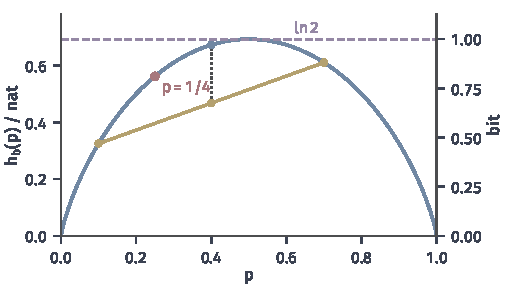
\includegraphics[width=86mm]{figures/07-probability/04-distribution-analysis/matplotlib/info-binary-entropy/figure.pdf}
  \caption{二元熵函数$h_{\mathrm{b}}(p)$（蓝），左轴nat、右轴bit。紫虚线为上界$\ln2$，在$p=\tfrac12$处达到。黄色弦连接$p=0.1$与$p=0.7$两点，其中点$0.470$低于曲线在$p=0.4$处的值$0.673$，体现凹性。红点为$p=\tfrac14$。}
  \label{fig:info-binary-entropy}
\end{BookInlineFigure}

图~\ref{fig:info-binary-entropy}中，$h_{\mathrm{b}}$在两端为零，对应确定的结果；在$p=\tfrac12$处取最大值$\ln2$，对应公平硬币；曲线关于$p=\tfrac12$对称，因为交换$0$与$1$不改变熵。端点附近曲线很陡：$h_{\mathrm{b}}'(p)=\ln\frac{1-p}{p}\to+\infty$（$p\downarrow0$），概率从$0$略微增加，熵增加得比概率快得多。第~\ref{sec:info-continuity}节讨论熵的连续性时会用到这一点。

三个取值的情形可以画在概率单纯形上。图~\ref{fig:info-simplex-entropy}中三角形的每个点是一张概率表，顶点是确定结果，中心是均匀分布。等熵线围绕中心形成一圈圈闭曲线：越靠近中心越不确定。

\begin{BookInlineFigure}
  \centering
  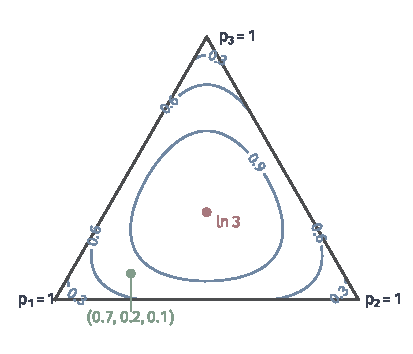
\includegraphics[width=70mm]{figures/07-probability/04-distribution-analysis/matplotlib/info-simplex-entropy/figure.pdf}
  \caption{三点分布$(p_1,p_2,p_3)$的熵在概率单纯形上的等值线（蓝，数值为nat）。顶点熵为$0$，红点为均匀分布，熵$\ln3\approx1.099$；绿点为$(0.7,0.2,0.1)$，熵约$0.802$ nat。超水平集$\{H\geq c\}$是凸集，对应熵的凹性。}
  \label{fig:info-simplex-entropy}
\end{BookInlineFigure}

\paragraph{可数取值}
取值可数无穷时，式~\eqref{eq:info-entropy}是非负项级数，可能收敛，也可能发散。几何分布$\operatorname{Geom}(\tfrac12)$取值$k=1,2,\dots$，概率$2^{-k}$，自信息$k\ln2$，于是
\[
  H(X)=\sum_{k\geq1}2^{-k}\,k\ln2=2\ln2,
\]
相当于平均问两题。

熵也可以是无穷。取$k\geq2$，$p_X(k)=c/(k(\ln k)^2)$，其中$c$使概率之和为$1$；由积分判别法，$\sum_{k\geq2}1/(k(\ln k)^2)$收敛，所以这样的$c>0$存在。这时
\[
  -\ln p_X(k)=\ln k+2\ln\ln k-\ln c\geq\ln k-\ln c.
\]
对充分大的$k$，$2\ln\ln k\geq0$，所以熵的级数从某项起不小于
\[
  \sum_k\frac{c}{k(\ln k)^2}\bigl(\ln k-\ln c\bigr)\geq\sum_k\frac{c}{k\ln k}-\ln c\sum_k\frac{c}{k(\ln k)^2},
\]
其中第一项发散，第二项有限，故$H(X)=+\infty$。这个分布的质量衰减得足够快，使概率之和有限，却不够快，使平均自信息有限。

所以定理~\ref{thm:info-entropy-range}的上界不能移用到可数字母表：$\ln m$随$m\to\infty$趋于无穷，并不给出有限上界。凹性在熵有限的分布之间仍然成立，因为证明只用到逐项的不等式；但涉及熵之差的公式，都要先核对相关的熵有限。

\subsection{微分熵}
\label{sec:info-differential-entropy}

连续随机变量的每个取值概率都是零，自信息全是无穷大，式~\eqref{eq:info-entropy}不能直接用。一个自然的替代是把概率质量换成密度：密度是单位长度上的概率质量，对密度取负对数再按分布平均。

\begin{definition}[微分熵]
\label{def:info-differential-entropy}
设随机变量$X$有密度$f_X$。若$f_X\ln f_X$在$\mathbb{R}$上可积，称
\begin{equation}
  h(X)=-\int_{\mathbb{R}}f_X(x)\ln f_X(x)\,\mathrm{d}x=\mathbb{E}[-\ln f_X(X)]
  \label{eq:info-differential-entropy}
\end{equation}
为$X$的\term{微分熵}（differential entropy），在$\{f_X=0\}$上约定被积函数为$0$。随机向量$\bm{X}$有联合密度时，同样定义$h(\bm{X})$。
\end{definition}

定义里要求$f_X\ln f_X$可积（即$f_X\lvert\ln f_X\rvert$的积分有限），是为了排除两种情形。离散熵的各项非负，最坏只是$+\infty$；而密度可以大于$1$，$-\ln f_X$有正有负，正部与负部的积分可能都发散，这时“$\infty-\infty$”没有意义。若只有一部分发散，可以约定$h(X)=+\infty$或$-\infty$，本章不使用这种扩展。

\paragraph{几个密度的微分熵}
均匀分布$\operatorname{Unif}(0,a)$的密度在$(0,a)$上为$1/a$，所以
\[
  h(X)=-\int_0^a\frac1a\ln\frac1a\,\mathrm{d}x=\ln a.
\]
$a<1$时它是负数。$\operatorname{Unif}(0,\tfrac12)$的微分熵是$-\ln2$，这不意味着“不确定性为负”，而是说密度$2$大于$1$。

正态分布$\mathcal{N}(\mu,\sigma^{2})$的对数密度是
\[
  \ln f_X(x)=-\frac12\ln(2\pi\sigma^{2})-\frac{(x-\mu)^{2}}{2\sigma^{2}}.
\]
取负号再按$X$平均，利用$\mathbb{E}[(X-\mu)^{2}]=\sigma^{2}$，得到
\begin{equation}
  h(X)=\frac12\ln(2\pi\sigma^{2})+\frac12=\frac12\ln(2\pi\mathrm{e}\sigma^{2}).
  \label{eq:info-gaussian-entropy}
\end{equation}
$\sigma=1$时约为$1.419$ nat。同样算出指数分布$\operatorname{Exp}(\lambda)$的微分熵：$-\ln f_X(x)=-\ln\lambda+\lambda x$，平均为$1-\ln\lambda$。

\paragraph{坐标尺度的作用}
把变量放大，密度就按比例变矮。设$a\neq0$，$Y=aX+b$，由第~\ref{chap:random-variable-transformations}章的换元公式，$f_Y(y)=f_X((y-b)/a)/\lvert a\rvert$。于是
\[
  -\ln f_Y(Y)=-\ln f_X(X)+\ln\lvert a\rvert,
\]
两边取期望，得到
\begin{equation}
  h(aX+b)=h(X)+\ln\lvert a\rvert.
  \label{eq:info-differential-entropy-scale}
\end{equation}
平移不改变微分熵，伸缩改变$\ln\lvert a\rvert$。图~\ref{fig:info-diff-entropy-scale}把这一点画了出来：宽度每加倍，高度减半，微分熵增加$\ln2$。

\begin{BookInlineFigure}
  \centering
  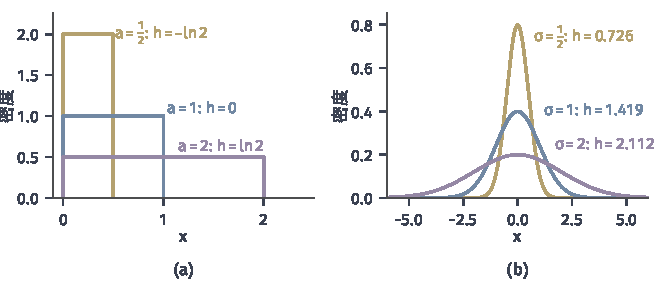
\includegraphics[width=112mm]{figures/07-probability/04-distribution-analysis/matplotlib/info-diff-entropy-scale/figure.pdf}
  \caption{微分熵随尺度变化。(a)$\operatorname{Unif}(0,a)$，$a=\tfrac12,1,2$（黄、蓝、紫），微分熵为$\ln a$。(b)$\mathcal{N}(0,\sigma^{2})$，$\sigma=\tfrac12,1,2$，微分熵按式~\eqref{eq:info-gaussian-entropy}计算，以nat计。宽度加倍时两组都增加$\ln2\approx0.693$。}
  \label{fig:info-diff-entropy-scale}
\end{BookInlineFigure}

式~\eqref{eq:info-differential-entropy-scale}揭示了微分熵与离散熵的根本不同。同一个长度用米记录是$X$，用厘米记录是$100X$，两者包含的关于这次测量的信息完全一样，微分熵却相差$\ln100$。离散熵没有这个问题：对取值作任何一一变换，概率表不变，熵不变。微分熵依赖坐标，只有在固定坐标下比较才有意义。更一般地，对严格单调可微的$g$，$Y=g(X)$满足$h(Y)=h(X)+\mathbb{E}[\ln\lvert g'(X)\rvert]$（右端各项有限时），推导与上面相同。

\paragraph{与量化后离散熵的关系}
微分熵可以从离散熵得到，只是要减去一个随精度增长的量。把实轴按宽度$\Delta>0$分成格子$[k\Delta,(k+1)\Delta)$，只记录$X$落在哪一格，得到离散变量$X_{\Delta}$，概率$p_k=\mathbb{P}(k\Delta\leq X<(k+1)\Delta)$。

若$f_X$连续，由积分中值定理，每格中有一点$\xi_k$使$p_k=f_X(\xi_k)\Delta$。代入离散熵并利用$\sum_kp_k=1$，得到
\[
  H(X_{\Delta})=-\sum_kf_X(\xi_k)\Delta\ln f_X(\xi_k)-\ln\Delta.
\]
右端第一项是$-\int f_X\ln f_X\,\mathrm{d}x$的一个Riemann和。若这个和在$\Delta\to0$时收敛到积分，就有
\begin{equation}
  H(X_{\Delta})+\ln\Delta\to h(X),\qquad\Delta\to0.
  \label{eq:info-quantized-entropy}
\end{equation}

$-\ln\Delta$是“把结果确定到精度$\Delta$”的代价：每把格子缩小一半，就要多回答一个是非题。连续结果要完全确定需要无穷多个是非题，离散熵趋于无穷；微分熵是减去这部分以后剩下的有限部分，所以它依赖格子的单位。$X\sim\operatorname{Unif}(0,1)$、$\Delta=1/n$时，$n$个格子等概率，$H(X_{\Delta})=\ln n$恰好等于$h(X)-\ln\Delta=0+\ln n$。

\begin{BookInlineFigure}
  \centering
  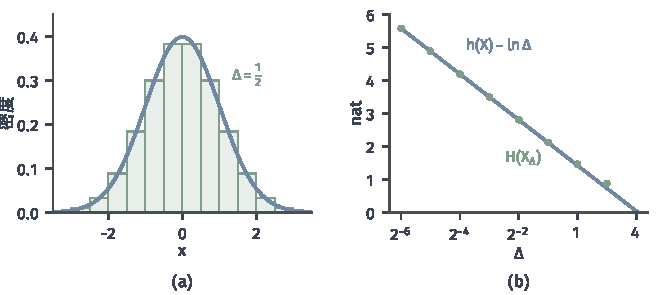
\includegraphics[width=112mm]{figures/07-probability/04-distribution-analysis/matplotlib/info-quantization/figure.pdf}
  \caption{标准正态变量的量化。(a)密度（蓝）与$\Delta=\tfrac12$时各格的概率除以格宽（浅绿柱）。(b)量化后离散熵$H(X_{\Delta})$的精确值（绿点）与$h(X)-\ln\Delta$（蓝线），$h(X)\approx1.419$ nat，横轴为对数刻度。差$H(X_{\Delta})+\ln\Delta-h(X)$在$\Delta=1,\tfrac12,\tfrac14$时约为$0.040,0.010,0.0026$。}
  \label{fig:info-quantization}
\end{BookInlineFigure}

图~\ref{fig:info-quantization}对标准正态变量逐格计算了$H(X_{\Delta})$。格子较宽时两者有可见的差距，$\Delta$每减半，差距约缩小为四分之一。

式~\eqref{eq:info-quantized-entropy}不是对任意密度都成立。上面的推导用到两件事：$f_X\ln f_X$的Riemann和收敛到积分，以及实轴无界时尾部格子的贡献可以忽略。密度连续且$f_X\ln f_X$在有界区间上Riemann可积时，有界区间上的部分成立；无界区间还需要控制尾部，读者可查阅~\scite{math-cover2006information}。密度剧烈振荡或尾部很重时，两边可能不相符。因此，微分熵与量化熵是两个不同的量，前者不是后者的极限值，而是后者减去$-\ln\Delta$后的极限，并且这个联系要单独核对条件。


\section{联合熵与条件熵}
\label{sec:info-joint-conditional}

有两个变量$X,Y$时，可以问两种问题：把有序对$(X,Y)$一起确定，平均要多少信息；已经知道$Y$以后，确定$X$还需要多少信息。前者只要把$(X,Y)$看成一个随机对象，后者要用条件分布。本节先分别定义这两个量，再说明它们怎样由“先揭示一个、再揭示另一个”的分解连接起来。

\subsection{联合熵}
\label{sec:info-joint-entropy}

有序对$(X,Y)$本身是一个离散随机对象，取值于$\mathcal{X}\times\mathcal{Y}$，联合概率质量$p_{X,Y}(x,y)$构成一张概率表。熵只依赖概率表，所以可以直接套用式~\eqref{eq:info-entropy}。

\begin{definition}[联合熵]
\label{def:info-joint-entropy}
离散随机变量$X,Y$的\term{联合熵}（joint entropy）是
\begin{equation}
  H(X,Y)=-\sum_{x,y}p_{X,Y}(x,y)\ln p_{X,Y}(x,y)=\mathbb{E}[-\ln p_{X,Y}(X,Y)].
  \label{eq:info-joint-entropy}
\end{equation}
多个变量的联合熵$H(X_1,\dots,X_n)$同样定义。若$(X,Y)$有联合密度$f_{X,Y}$，在$f_{X,Y}\lvert\ln f_{X,Y}\rvert$可积时，联合微分熵$h(X,Y)$定义为$-\iint f_{X,Y}\ln f_{X,Y}\,\mathrm{d}x\,\mathrm{d}y$。
\end{definition}

联合熵并不由两个边缘分布决定。图~\ref{fig:info-same-marginals}的三张表，$X$与$Y$的边缘都是公平硬币，$H(X)=H(Y)=\ln2$。独立时四格各$\tfrac14$，联合熵是$\ln4\approx1.386$ nat，正好是$H(X)+H(Y)$。$Y=X$时只有对角线两格有质量，联合熵只有$\ln2$：知道$X$就知道$Y$，有序对并不比单个变量更难确定。第三张表是公平硬币经过以概率$\tfrac14$出错的线路，
\[
  H(X,Y)=-2\cdot\tfrac38\ln\tfrac38-2\cdot\tfrac18\ln\tfrac18\approx1.255\ \mathrm{nat},
\]
介于前两者之间。

\begin{BookInlineFigure}
  \centering
  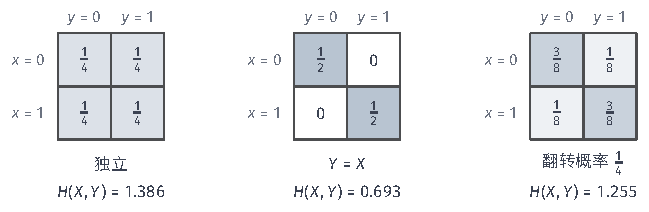
\includegraphics[width=109.8mm]{figures/07-probability/04-distribution-analysis/tikz/info-same-marginals/figure.pdf}
  \caption{三张边缘都是$(\tfrac12,\tfrac12)$的联合概率表，格中数值为$p_{X,Y}(x,y)$，底色越深质量越大。联合熵（nat）随依赖关系改变：独立时最大，$Y=X$时最小，以概率$\tfrac14$翻转时居中。}
  \label{fig:info-same-marginals}
\end{BookInlineFigure}

三张表的共同点是$H(X,Y)\leq H(X)+H(Y)$，独立时取等号；这个不等式在第~\ref{sec:info-mi-entropy}节证明。它说明依赖关系只会让整体更容易确定：一部分不确定性被两个变量“共享”了，不必重复计算。

联合微分熵的例子是二元正态分布。若$\bm{X}\sim\mathcal{N}(\bm{\mu},\bm{\Sigma})$是$d$维正态向量，协方差矩阵$\bm{\Sigma}$正定，对数密度为
\[
  \ln f(\bm{x})=-\frac12\ln\bigl((2\pi)^{d}\det\bm{\Sigma}\bigr)-\frac12(\bm{x}-\bm{\mu})^{\top}\bm{\Sigma}^{-1}(\bm{x}-\bm{\mu}).
\]
二次型的期望是$\operatorname{tr}(\bm{\Sigma}^{-1}\bm{\Sigma})=d$，所以
\begin{equation}
  h(\bm{X})=\frac12\ln\bigl((2\pi\mathrm{e})^{d}\det\bm{\Sigma}\bigr).
  \label{eq:info-gaussian-vector-entropy}
\end{equation}
二维标准化、相关系数为$\rho$时$\det\bm{\Sigma}=1-\rho^{2}$，相关越强，联合微分熵越小，$\lvert\rho\rvert\to1$时趋于$-\infty$。质量越来越集中到一条直线附近，平面上的密度越来越高。

\subsection{条件熵}
\label{sec:info-conditional-entropy}

已知$Y=y$以后，$X$的概率表变成条件分布$p_{X\mid Y}(\cdot\mid y)$：条件化就是只保留$Y=y$的那一列，再重新归一。这张新表的熵，是看到$Y=y$以后$X$剩下的不确定性。不同的$y$留下的不确定性不同，再按$y$出现的概率平均。

\begin{definition}[条件熵]
\label{def:info-conditional-entropy}
设$X,Y$是离散随机变量。对$p_Y(y)>0$的$y$，令
\begin{equation}
  H(X\mid Y=y)=-\sum_xp_{X\mid Y}(x\mid y)\ln p_{X\mid Y}(x\mid y).
  \label{eq:info-conditional-entropy-value}
\end{equation}
$X$在给定$Y$时的\term{条件熵}（conditional entropy）是
\begin{equation}
  H(X\mid Y)=\sum_{y}p_Y(y)\,H(X\mid Y=y)=\mathbb{E}\bigl[-\ln p_{X\mid Y}(X\mid Y)\bigr].
  \label{eq:info-conditional-entropy}
\end{equation}
\end{definition}

式~\eqref{eq:info-conditional-entropy}中第一个和是对式~\eqref{eq:info-conditional-entropy-value}的平均。第二个等号把双重求和合并：$p_Y(y)p_{X\mid Y}(x\mid y)=p_{X,Y}(x,y)$，所以
\[
  H(X\mid Y)=-\sum_{x,y}p_{X,Y}(x,y)\ln p_{X\mid Y}(x\mid y),
\]
各项非负，求和次序可以交换。条件熵是平均剩余不确定性，不是对某一个观测值的保证。

\paragraph{一张不对称的表}
下面这张表在后面几节反复使用：
\begin{equation}
  p_{X,Y}(0,0)=\tfrac14,\quad p_{X,Y}(0,1)=0,\quad p_{X,Y}(1,0)=\tfrac38,\quad p_{X,Y}(1,1)=\tfrac38.
  \label{eq:info-z-table}
\end{equation}
可以把它想成：$X=0$时$Y$必为$0$；$X=1$时$Y$是一枚公平硬币。边缘分布为
\[
  p_X=(\tfrac14,\tfrac34),\qquad p_Y=(\tfrac58,\tfrac38).
\]

按行看，$X=0$那一行条件分布是$(1,0)$，熵为$0$；$X=1$那一行是$(\tfrac12,\tfrac12)$，熵为$\ln2$。按$p_X$平均，
\[
  H(Y\mid X)=\tfrac14\cdot0+\tfrac34\ln2\approx0.520\ \mathrm{nat}.
\]

按列看，$Y=0$那一列的条件分布是$(\tfrac14,\tfrac38)/\tfrac58=(\tfrac25,\tfrac35)$，熵为$h_{\mathrm{b}}(\tfrac25)\approx0.673$；$Y=1$那一列是$(0,1)$，熵为$0$。按$p_Y$平均，
\[
  H(X\mid Y)=\tfrac58\cdot0.673+\tfrac38\cdot0\approx0.421\ \mathrm{nat}.
\]
两个条件熵不相等：条件熵与“谁给定谁”有关。

\begin{BookInlineFigure}
  \centering
  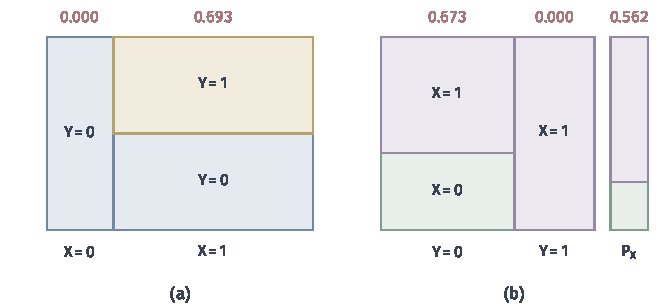
\includegraphics[width=112mm]{figures/07-probability/04-distribution-analysis/matplotlib/info-conditional-slices/figure.pdf}
  \caption{表~\eqref{eq:info-z-table}的条件分布。(a)按$X$分割，宽度为$p_X(x)$，高度为$Y$的条件概率，红色数字为各行的条件熵$H(Y\mid X=x)$。(b)按$Y$分割，宽度正比于$p_Y(y)$，高度为$X$的条件概率，红色数字为$H(X\mid Y=y)$；最右的窄条是无条件的$p_X$及其熵$H(X)\approx0.562$。单位为nat。}
  \label{fig:info-conditional-slices}
\end{BookInlineFigure}

图~\ref{fig:info-conditional-slices}(b)还显示了一个容易误解的现象：$H(X\mid Y=0)\approx0.673$大于$H(X)\approx0.562$。观测到$Y=0$以后，$X$反而更不确定了，因为$Y=0$把原来偏向$X=1$的质量拉向均匀。但这样的观测值只是一部分；$Y=1$时$X$完全确定。平均以后$H(X\mid Y)\approx0.421$，仍小于$H(X)$。第~\ref{sec:info-mi-entropy}节证明这对一切离散变量成立：条件化平均来说不增加熵，但单个观测值可以增加。

\paragraph{离散与连续的区别}
离散时$H(X\mid Y=y)\geq0$，所以$H(X\mid Y)\geq0$，等号当且仅当每个$y$下$X$确定，即$X$是$Y$的函数（除去零概率的$y$）。连续时用条件密度代替条件概率，定义
\[
  h(X\mid Y)=-\iint f_{X,Y}(x,y)\ln f_{X\mid Y}(x\mid y)\,\mathrm{d}x\,\mathrm{d}y,
\]
要求条件密度存在且被积函数绝对可积。它和微分熵一样可以为负，也依赖坐标。

二元标准正态、相关系数$\rho$时，给定$X=x$，$Y$的条件分布是$\mathcal{N}(\rho x,1-\rho^{2})$，与$x$有关的只有均值。每个条件分布的微分熵相同，由式~\eqref{eq:info-gaussian-entropy}，
\begin{equation}
  h(Y\mid X)=\frac12\ln\bigl(2\pi\mathrm{e}(1-\rho^{2})\bigr).
  \label{eq:info-gaussian-conditional-entropy}
\end{equation}
$\rho=0.9$时它约为$0.589$ nat；$\rho^{2}>1-1/(2\pi\mathrm{e})\approx0.941$时它为负数。负值只说明条件密度很窄，不能读成“剩余不确定性为负”。

\subsection{熵的链式法则}
\label{sec:info-entropy-chain-rule}

确定$(X,Y)$可以分两步：先确定$X$，再在已知$X$的情况下确定$Y$。图~\ref{fig:info-chain-tree}把表~\eqref{eq:info-z-table}画成两步的树。第一步的不确定性是$H(X)\approx0.562$；第二步要看走到哪一支，$X=0$那支已无悬念，$X=1$那支还剩$\ln2$，平均$0.520$。两步合起来应当是整体的不确定性。

\begin{BookInlineFigure}
  \centering
  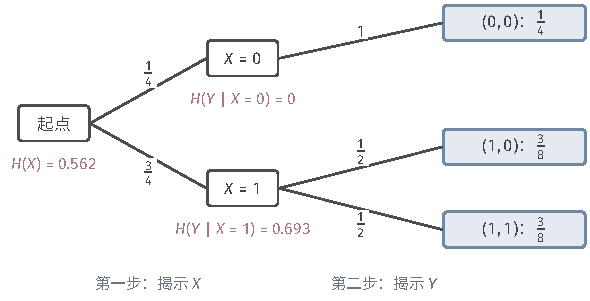
\includegraphics[width=100mm]{figures/07-probability/04-distribution-analysis/tikz/info-chain-tree/figure.pdf}
  \caption{表~\eqref{eq:info-z-table}的两步揭示树。第一步按$p_X=(\tfrac14,\tfrac34)$揭示$X$，第二步按条件分布揭示$Y$；叶子为联合概率。红字为各步的熵（nat），第二步的平均为$\tfrac34\ln2\approx0.520$，与第一步的$0.562$相加得$H(X,Y)\approx1.082$。}
  \label{fig:info-chain-tree}
\end{BookInlineFigure}

\begin{theorem}[熵的链式法则]
\label{thm:info-entropy-chain-rule}
设$X,Y$是离散随机变量，则在$[0,\infty]$中
\begin{equation}
  H(X,Y)=H(X)+H(Y\mid X).
  \label{eq:info-entropy-chain-rule}
\end{equation}
对离散随机变量$X_1,\dots,X_n$，
\begin{equation}
  H(X_1,\dots,X_n)=\sum_{i=1}^{n}H(X_i\mid X_1,\dots,X_{i-1}),
  \label{eq:info-entropy-chain-rule-n}
\end{equation}
其中$i=1$的项理解为$H(X_1)$。
\end{theorem}

\begin{proof}
在$p_{X,Y}(x,y)>0$的点，$p_{X,Y}(x,y)=p_X(x)\,p_{Y\mid X}(y\mid x)$，取负对数，得到
\[
  -\ln p_{X,Y}(x,y)=-\ln p_X(x)-\ln p_{Y\mid X}(y\mid x).
\]
右端两项都非负。乘以$p_{X,Y}(x,y)$后对$(x,y)$求和；非负项的和可以拆开、可以交换次序，即使为$+\infty$也成立。第一项的和是$-\sum_xp_X(x)\ln p_X(x)=H(X)$，第二项的和由式~\eqref{eq:info-conditional-entropy}是$H(Y\mid X)$。

多个变量时，把$(X_1,\dots,X_{n-1})$看成一个变量，对它与$X_n$用式~\eqref{eq:info-entropy-chain-rule}，得到
\[
  H(X_1,\dots,X_n)=H(X_1,\dots,X_{n-1})+H(X_n\mid X_1,\dots,X_{n-1}),
\]
再对前一项归纳即可。
\end{proof}

用表~\eqref{eq:info-z-table}验证。直接计算联合熵，
\[
  H(X,Y)=-\tfrac14\ln\tfrac14-2\cdot\tfrac38\ln\tfrac38\approx1.082.
\]
先揭示$X$，$H(X)+H(Y\mid X)\approx0.562+0.520=1.082$。换一个顺序，$H(Y)=h_{\mathrm{b}}(\tfrac38)\approx0.662$，$H(Y)+H(X\mid Y)\approx0.662+0.421=1.082$，也相同。揭示的顺序不同，每一步分到的不确定性不同，总量不变。

链式法则不要求独立。变量独立时，$p_{X_i\mid X_1,\dots,X_{i-1}}=p_{X_i}$，各条件熵等于无条件熵，式~\eqref{eq:info-entropy-chain-rule-n}化为$\sum_iH(X_i)$。不独立时不能把联合熵写成边缘熵之和，图~\ref{fig:info-same-marginals}已经给出了反例。

\paragraph{移项与连续情形}
链式法则常被移项为$H(Y\mid X)=H(X,Y)-H(X)$。这只在$H(X)<\infty$时有意义；否则右端可能是$\infty-\infty$。例如取$H(X)=\infty$的可数变量并令$Y=X$，$H(X,Y)=\infty$，$H(Y\mid X)=0$，链式法则$\infty=\infty+0$成立，移项却没有意义。

对有联合密度的$(X,Y)$，同样有$f_{X,Y}=f_X\,f_{Y\mid X}$，取负对数后积分，得到
\[
  h(X,Y)=h(X)+h(Y\mid X).
\]
但这里各项可以为负，不能像离散时那样靠“非负项可以拆开”保证等式。需要先核对$f_X\lvert\ln f_X\rvert$与$f_{X,Y}\lvert\ln f_{Y\mid X}\rvert$都可积，这时拆开积分合法，等式成立，并且$h(X,Y)$也有限。二元正态是一个检查的例子：由式~\eqref{eq:info-gaussian-entropy}与式~\eqref{eq:info-gaussian-conditional-entropy}，
\[
  h(X)+h(Y\mid X)=\frac12\ln(2\pi\mathrm{e})+\frac12\ln\bigl(2\pi\mathrm{e}(1-\rho^{2})\bigr),
\]
与式~\eqref{eq:info-gaussian-vector-entropy}在$d=2$、$\det\bm{\Sigma}=1-\rho^{2}$时的值相同。


\section{互信息}
\label{sec:info-mutual-information}

公平硬币$X$经过以概率$\tfrac14$出错的线路得到$Y$。看到$Y$之前，$X$的不确定性是$\ln2$；看到$Y$以后，平均剩下$H(X\mid Y)=h_{\mathrm{b}}(\tfrac14)\approx0.562$。两者之差约$0.131$ nat，是观测$Y$平均消除的不确定性。这个差可以作为“$Y$含有多少关于$X$的信息”。

但熵之差只在熵有限、并且两个变量都是离散时才写得出来。连续变量的微分熵依赖坐标，一个变量离散、另一个连续时还会出现某一项根本没有定义的情形。本节换一个出发点：$X$与$Y$不相关联，就是联合分布等于边缘分布的乘积；联合分布偏离这个乘积的程度，用KL散度衡量。这个定义对任何取值空间都有意义，熵之差是它在条件满足时的一种算法。

\subsection{定义与独立性}
\label{sec:info-mi-definition}

先回顾第~\ref{chap:distribution-comparison}章的KL散度。设$P,Q$是同一可测空间上的概率分布。若$P\ll Q$，记$r=\mathrm{d}P/\mathrm{d}Q$，则
\begin{equation}
  D_{\mathrm{KL}}(P\Vert Q)=\int\ln r\,\mathrm{d}P\in[0,+\infty];
  \label{eq:info-kl-recall}
\end{equation}
若$P$不绝对连续于$Q$，则$D_{\mathrm{KL}}(P\Vert Q)=+\infty$。$\ln r$的负部总对$P$可积，所以积分总有意义；KL散度非负，并且为零当且仅当$P=Q$。离散时$r(x)=p(x)/q(x)$，式~\eqref{eq:info-kl-recall}化为$\sum_xp(x)\ln\frac{p(x)}{q(x)}$。

\begin{definition}[互信息]
\label{def:info-mutual-information}
设随机变量（或随机元素）$X,Y$的联合分布为$P_{X,Y}$，边缘分布为$P_X,P_Y$。$X$与$Y$的\term{互信息}（mutual information）是
\begin{equation}
  I(X;Y)=D_{\mathrm{KL}}\bigl(P_{X,Y}\Vert P_X\otimes P_Y\bigr)\in[0,+\infty].
  \label{eq:info-mutual-information}
\end{equation}
离散时
\begin{equation}
  I(X;Y)=\sum_{x,y}p_{X,Y}(x,y)\ln\frac{p_{X,Y}(x,y)}{p_X(x)\,p_Y(y)}.
  \label{eq:info-mutual-information-discrete}
\end{equation}
\end{definition}

$P_X\otimes P_Y$是“边缘不变、但把两个变量拆成独立”所得的分布。互信息比较真实的联合规律与这个独立参照，差异全部来自依赖关系，因为两者的边缘完全相同。

\begin{theorem}[互信息的基本性质]
\label{thm:info-mi-basic}
对任意随机元素$X,Y$：
\begin{enumerate}
  \item $I(X;Y)\geq0$；
  \item $I(X;Y)=I(Y;X)$；
  \item $I(X;Y)=0$当且仅当$X$与$Y$独立。
\end{enumerate}
\end{theorem}

\begin{proof}
第一条和第三条是KL散度的非负性及其零值条件：$I(X;Y)=0$当且仅当$P_{X,Y}=P_X\otimes P_Y$，而这正是第~\ref{chap:probability-spaces}章中独立的定义。

第二条用交换坐标的映射$\sigma(x,y)=(y,x)$。它把$P_{X,Y}$推前为$P_{Y,X}$，把$P_X\otimes P_Y$推前为$P_Y\otimes P_X$。若$P_{X,Y}\ll P_X\otimes P_Y$，密度为$r$，则$r\circ\sigma^{-1}$是推前后两个分布之间的密度，按推前测度的积分换元，两个KL的积分相等；若不绝对连续，推前后同样不绝对连续，两边都是$+\infty$。
\end{proof}

第三条比“协方差为零”强得多。取$X$在$\{-1,0,1\}$上均匀，$Y=X^{2}$：$\operatorname{Cov}(X,Y)=\mathbb{E}[X^{3}]=0$，但$Y$由$X$确定，下一小节会算出$I(X;Y)\approx0.637>0$。互信息为零能排除一切形式的依赖，零协方差只能排除线性部分。

\paragraph{二元例子}
用式~\eqref{eq:info-mutual-information-discrete}计算出错线路的例子。联合表是对角$\tfrac38$、非对角$\tfrac18$，边缘乘积处处$\tfrac14$，比值分别为$\tfrac32$与$\tfrac12$。于是
\[
  I(X;Y)=2\cdot\tfrac38\ln\tfrac32+2\cdot\tfrac18\ln\tfrac12=\tfrac34\ln\tfrac32-\tfrac14\ln2\approx0.1308\ \mathrm{nat},
\]
约$0.189$ bit。对角格的比值大于$1$，说明“相同”比独立时更常见；非对角格的比值小于$1$，对数为负，但按$P_{X,Y}$加权后总和非负。

\paragraph{互信息可以为无穷}
定义允许$I(X;Y)=+\infty$，这不是边缘情形。设$X\sim\operatorname{Unif}(0,1)$，$Y=X$。联合分布全部集中在对角线$D=\{(x,x)\}$上，$P_{X,Y}(D)=1$；而
\[
  (P_X\otimes P_Y)(D)=\int_0^1P_Y(\{x\})\,\mathrm{d}x=0.
\]
$P_{X,Y}$不绝对连续于$P_X\otimes P_Y$，所以$I(X;Y)=+\infty$。一个连续变量完全知道另一个连续变量，等于知道了无穷多位小数。离散时也会出现无穷：若$H(X)=+\infty$，令$Y=X$，下一小节会得到$I(X;Y)=H(X)=+\infty$。

定义也不要求任何密度。联合分布可以没有联合密度，比如上面集中在对角线上的分布；只要$P_{X,Y}\ll P_X\otimes P_Y$，KL就由密度比计算，否则直接为无穷。

\subsection{与熵的关系}
\label{sec:info-mi-entropy}

回到章首的说法：互信息是观测带来的不确定性的减少。下面的定理说明，离散情形下只要相关的熵有限，两种说法一致。

\begin{theorem}[互信息与熵]
\label{thm:info-mi-entropy}
设$X,Y$是离散随机变量。若$H(X)<\infty$，则$H(X\mid Y)\leq H(X)$，并且
\begin{equation}
  I(X;Y)=H(X)-H(X\mid Y).
  \label{eq:info-mi-entropy-difference}
\end{equation}
若$H(X)$与$H(Y)$都有限，则$H(X,Y)$有限，并且
\begin{equation}
  I(X;Y)=H(X)+H(Y)-H(X,Y).
  \label{eq:info-mi-entropy-sum}
\end{equation}
\end{theorem}

\begin{proof}
在$p_{X,Y}(x,y)>0$的点，把比值中的$p_{X,Y}/p_Y$写成条件概率，
\[
  \ln\frac{p_{X,Y}(x,y)}{p_X(x)p_Y(y)}=\bigl(-\ln p_X(x)\bigr)-\bigl(-\ln p_{X\mid Y}(x\mid y)\bigr).
\]
记$A=-\ln p_X(X)$，$B=-\ln p_{X\mid Y}(X\mid Y)$。两者非负，期望分别为
\[
  \mathbb{E}[A]=H(X)<\infty,\qquad\mathbb{E}[B]=H(X\mid Y).
\]由式~\eqref{eq:info-mutual-information-discrete}，$I(X;Y)=\mathbb{E}[A-B]$。$A$可积而$B\geq0$，期望可以拆开，得到
\[
  I(X;Y)=\mathbb{E}[A]-\mathbb{E}[B]=H(X)-H(X\mid Y).
\]
互信息非负，所以$H(X\mid Y)\leq H(X)$，右端是两个有限数之差。

第二个等式由链式法则得到：$H(Y)<\infty$时由第一部分$H(X\mid Y)\leq H(X)<\infty$，式~\eqref{eq:info-entropy-chain-rule}给出$H(X,Y)=H(Y)+H(X\mid Y)$有限，代入式~\eqref{eq:info-mi-entropy-difference}即得。
\end{proof}

由对称性，同样有$I(X;Y)=H(Y)-H(Y\mid X)$（$H(Y)<\infty$时）。这几个关系有三个直接推论，都在相应熵有限时成立：
\begin{itemize}
  \item \textbf{条件化平均不增加熵}：$H(X\mid Y)\leq H(X)$，等号当且仅当$X,Y$独立。上一节的表~\eqref{eq:info-z-table}说明，这个结论只对平均成立，对单个观测值$H(X\mid Y=0)$可以大于$H(X)$。
  \item \textbf{联合熵的次可加性}：$H(X,Y)\leq H(X)+H(Y)$，这正是图~\ref{fig:info-same-marginals}中观察到的。
  \item \textbf{上界}：$I(X;Y)\leq\min\{H(X),H(Y)\}$，并且$I(X;X)=H(X)$，因为$H(X\mid X)=0$。离散变量与自身的互信息就是它的熵，熵因此也叫“自身信息”。
\end{itemize}

$Y=X^{2}$的例子中，$Y$是$X$的函数，$H(Y\mid X)=0$，所以$I(X;Y)=H(Y)$；$Y$取$1$的概率是$\tfrac23$，$H(Y)=h_{\mathrm{b}}(\tfrac13)\approx0.637$。

\begin{BookInlineFigure}
  \centering
  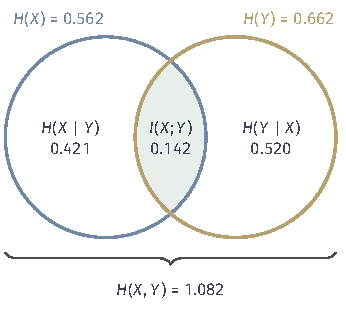
\includegraphics[width=58.5mm]{figures/07-probability/04-distribution-analysis/tikz/info-venn/figure.pdf}
  \caption{两个离散变量的熵与互信息的记账图，数值（nat）取自表~\eqref{eq:info-z-table}。蓝圈表示$H(X)$，黄圈表示$H(Y)$，重叠部分（浅绿）表示$I(X;Y)$，两圈之外的部分分别是条件熵，两圈的并表示$H(X,Y)$。图只表示有限熵之间的加减关系，面积不是测度。}
  \label{fig:info-venn}
\end{BookInlineFigure}

图~\ref{fig:info-venn}把这些关系画成两个重叠的圆。表~\eqref{eq:info-z-table}给出
\[
  I(X;Y)=H(X)-H(X\mid Y)\approx0.562-0.421=0.142,
\]
也等于$H(Y)-H(Y\mid X)\approx0.662-0.520=0.142$。图很方便记忆，但它只是有限熵之间的记账：三个变量时，三圈公共部分对应的量可以为负（第~\ref{sec:info-mi-chain-rule}节的异或例子），连续变量时各块可以为负，不能把它当成真正的面积。

再看出错线路的例子随出错概率$\varepsilon$的变化。$H(X)=\ln2$不变，$H(X\mid Y)=h_{\mathrm{b}}(\varepsilon)$，所以
\[
  I(X;Y)=\ln2-h_{\mathrm{b}}(\varepsilon).
\]
图~\ref{fig:info-bsc-curves}中两条曲线之和始终是$\ln2$。$\varepsilon=0$时观测完全揭示$X$；$\varepsilon=\tfrac12$时$Y$与$X$独立，互信息为零；$\varepsilon=1$时线路总是出错，把$Y$翻转回来就完全知道$X$，互信息又回到$\ln2$。互信息衡量的是能否从$Y$推出$X$，不是$Y$与$X$是否相等。

\begin{BookInlineFigure}
  \centering
  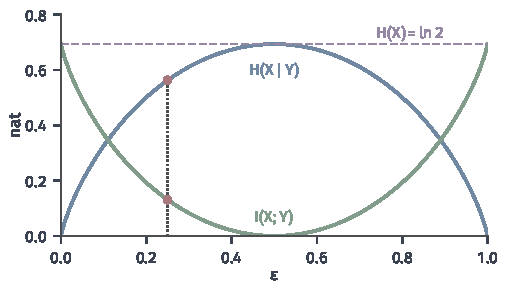
\includegraphics[width=86mm]{figures/07-probability/04-distribution-analysis/matplotlib/info-bsc-curves/figure.pdf}
  \caption{公平硬币$X$经以概率$\varepsilon$出错的线路得到$Y$。蓝线为$H(X\mid Y)=h_{\mathrm{b}}(\varepsilon)$，绿线为$I(X;Y)=\ln2-h_{\mathrm{b}}(\varepsilon)$，紫虚线为$H(X)=\ln2$，单位nat。红点为$\varepsilon=\tfrac14$：$0.562$与$0.131$。}
  \label{fig:info-bsc-curves}
\end{BookInlineFigure}

\paragraph{连续情形}
$(X,Y)$有联合密度时，若$h(Y)$与$h(Y\mid X)$都有限，同样的推导（把求和换成积分，拆开的依据是两项都绝对可积）给出
\[
  I(X;Y)=h(Y)-h(Y\mid X).
\]
二元标准正态由式~\eqref{eq:info-gaussian-entropy}与式~\eqref{eq:info-gaussian-conditional-entropy}得到
\begin{equation}
  I(X;Y)=\frac12\ln(2\pi\mathrm{e})-\frac12\ln\bigl(2\pi\mathrm{e}(1-\rho^{2})\bigr)=-\frac12\ln(1-\rho^{2}).
  \label{eq:info-gaussian-mi}
\end{equation}
$\rho=0.9$时约$0.830$ nat；$\lvert\rho\rvert\to1$时趋于无穷，与上面$Y=X$的例子一致。两个微分熵各自依赖坐标，相减后的互信息不依赖：分别把$X,Y$作伸缩，式~\eqref{eq:info-differential-entropy-scale}中的$\ln\lvert a\rvert$在两项中相消。

\begin{BookInlineFigure}
  \centering
  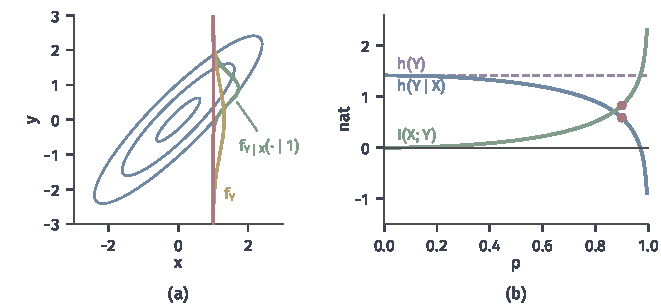
\includegraphics[width=112mm]{figures/07-probability/04-distribution-analysis/matplotlib/info-gaussian-mi/figure.pdf}
  \caption{二元标准正态分布。(a)$\rho=0.9$时联合密度的等值线（蓝）；红线为$x=1$，绿线为$Y$在$X=1$下的条件密度$\mathcal{N}(0.9,0.19)$，黄线为$Y$的边缘密度$\mathcal{N}(0,1)$，均横向画出。(b)$h(Y)$（紫虚线）、$h(Y\mid X)$（蓝）与$I(X;Y)$（绿）随$\rho$的变化，单位nat；红点为$\rho=0.9$时的$0.589$与$0.830$。}
  \label{fig:info-gaussian-mi}
\end{BookInlineFigure}

图~\ref{fig:info-gaussian-mi}(a)是熵差的直观来源：条件密度比边缘密度窄得多，宽度之比的对数就是减少的不确定性。(b)中$h(Y\mid X)$在$\rho$接近$1$时变为负数，而互信息始终非负。

熵差公式需要的熵可能不存在，互信息却仍有定义。设$X$等可能取$\pm1$，$Z\sim\mathcal{N}(0,1)$与$X$独立，$Y=X+Z$。$X$是离散的，没有密度，$h(X)$与$h(X\mid Y)$都没有定义，“$h(X)-h(X\mid Y)$”写不出来。但给定$X=x$时$Y$的条件密度是$\varphi(y-x)$，$h(Y\mid X)=\tfrac12\ln(2\pi\mathrm{e})$；$Y$的密度是两个正态密度的平均，方差为$2$，$h(Y)$有限。于是
\[
  I(X;Y)=h(Y)-h(Y\mid X)
\]
是一个有限的正数。所以，熵差是在各项有意义时计算互信息的工具，而式~\eqref{eq:info-mutual-information}才是定义。

\subsection{条件互信息}
\label{sec:info-conditional-mi}

已经知道第三个变量$Z$时，$X$与$Y$之间还剩多少共享信息？做法与条件熵相同：固定$Z=z$，在条件分布下计算互信息，再按$Z$的分布平均。连续的$Z$要用第~\ref{chap:conditional-distributions}章的正则条件分布，才能对每个$z$谈论“给定$Z=z$时$(X,Y)$的分布”。

\begin{definition}[条件互信息]
\label{def:info-conditional-mi}
设$X,Y,Z$取值于标准Borel空间，于是$(X,Y)$给定$Z$的正则条件分布$P_{X,Y\mid Z}(\cdot\mid z)$存在，记其边缘为$P_{X\mid Z}(\cdot\mid z)$、$P_{Y\mid Z}(\cdot\mid z)$。$X$与$Y$在给定$Z$时的\term{条件互信息}（conditional mutual information）是
\begin{equation}
  I(X;Y\mid Z)=\int D_{\mathrm{KL}}\bigl(P_{X,Y\mid Z}(\cdot\mid z)\Vert P_{X\mid Z}(\cdot\mid z)\otimes P_{Y\mid Z}(\cdot\mid z)\bigr)\,P_Z(\mathrm{d}z).
  \label{eq:info-conditional-mi}
\end{equation}
离散时
\begin{equation}
  I(X;Y\mid Z)=\sum_{x,y,z}p_{X,Y,Z}(x,y,z)\ln\frac{p_{X,Y\mid Z}(x,y\mid z)}{p_{X\mid Z}(x\mid z)\,p_{Y\mid Z}(y\mid z)}.
  \label{eq:info-conditional-mi-discrete}
\end{equation}
\end{definition}

被积函数是$z$的非负可测函数，积分在$[0,+\infty]$中总有意义。正则条件分布只在$P_Z$几乎处处的意义下唯一，换一个版本只在零概率的$z$上改变被积函数，积分不变。没有标准Borel这类条件时，正则条件分布可能不存在，式~\eqref{eq:info-conditional-mi}就不能这样写。

\begin{theorem}[条件互信息与条件独立]
\label{thm:info-conditional-mi-zero}
在定义~\ref{def:info-conditional-mi}的条件下，$I(X;Y\mid Z)\geq0$；$I(X;Y\mid Z)=0$当且仅当$X$与$Y$在给定$Z$时条件独立。
\end{theorem}

\begin{proof}
被积函数是KL散度，非负，所以积分非负。非负函数的积分为零，当且仅当它对$P_Z$几乎处处为零；由KL的零值条件，这就是对几乎所有$z$，
\[
  P_{X,Y\mid Z}(\cdot\mid z)=P_{X\mid Z}(\cdot\mid z)\otimes P_{Y\mid Z}(\cdot\mid z).
\]按第~\ref{chap:conditional-distributions}章，这正是给定$Z$时的条件独立。
\end{proof}

在离散且$H(X\mid Z)<\infty$时，把定理~\ref{thm:info-mi-entropy}的证明逐个条件值地做一遍，得到
\begin{equation}
  I(X;Y\mid Z)=H(X\mid Z)-H(X\mid Y,Z).
  \label{eq:info-conditional-mi-entropy}
\end{equation}
它是在已经知道$Z$的前提下，再观测$Y$所减少的关于$X$的不确定性。

条件互信息与互信息是两个不同的量，下一小节的例子说明两者之间没有固定的大小关系。

\subsection{互信息的链式法则}
\label{sec:info-mi-chain-rule}

一组观测$(Y,Z)$提供的关于$X$的信息，可以分两步获得：先看$Y$，得到$I(X;Y)$；再看$Z$，新增的是已知$Y$时$Z$还能提供的信息$I(X;Z\mid Y)$。

\begin{theorem}[互信息的链式法则]
\label{thm:info-mi-chain-rule}
设$X,Y,Z$取值于标准Borel空间，则在$[0,+\infty]$中
\begin{equation}
  I(X;Y,Z)=I(X;Y)+I(X;Z\mid Y).
  \label{eq:info-mi-chain-rule}
\end{equation}
一般地，
\begin{equation}
  I(X;Y_1,\dots,Y_n)=\sum_{i=1}^{n}I(X;Y_i\mid Y_1,\dots,Y_{i-1}).
  \label{eq:info-mi-chain-rule-n}
\end{equation}
\end{theorem}

\begin{proof}
先证离散且$H(X)<\infty$的情形。由式~\eqref{eq:info-mi-entropy-difference}及其条件形式~\eqref{eq:info-conditional-mi-entropy}，
\[
  I(X;Y,Z)=H(X)-H(X\mid Y,Z),\qquad I(X;Y)=H(X)-H(X\mid Y),
\]
以及
\[
  I(X;Z\mid Y)=H(X\mid Y)-H(X\mid Y,Z).
\]
三个式子里的熵都不超过$H(X)$，都是有限数。后两式相加，$H(X\mid Y)$相消，得到第一式。

一般情形不能假定熵有限，要直接分解KL散度。在离散情形，对一切三元组有
\[
  \frac{p_{X,Y,Z}}{p_X\,p_{Y,Z}}=\frac{p_{X,Y}}{p_X\,p_Y}\cdot\frac{p_{X,Z\mid Y}}{p_{X\mid Y}\,p_{Z\mid Y}},
\]
等式两边分子分母都按$p_{X,Y,Z}=p_{X,Y}\,p_{Z\mid X,Y}$与$p_{Y,Z}=p_Y\,p_{Z\mid Y}$展开即可核对。取对数后按$P_{X,Y,Z}$平均，第一个因子给出$I(X;Y)$，第二个给出$I(X;Z\mid Y)$。在一般空间，这一步是KL散度对联合分布的分解：两个联合分布的KL等于边缘的KL加上条件分布KL的平均。把两项的平均拆开、并允许取$+\infty$，需要用到对数比负部的可积性与正则条件分布的可测性，推导较长，这里只用它的结论。

多个观测时对$n$归纳：把$(Y_1,\dots,Y_{n-1})$看成一个变量，对它与$Y_n$用式~\eqref{eq:info-mi-chain-rule}。
\end{proof}

一般空间中KL散度分解的完整论证，读者可查阅~\scite{math-cover2006information}。

链式法则说明，信息可以按观测的先后分批记账，与熵的链式法则平行。不过，下面两个例子说明，第二步的条件互信息可以比无条件的互信息大，也可以小。

\paragraph{条件化可以增加互信息}
设$X,Y$是独立的公平硬币，$Z=X\oplus Y$为异或（相同为$0$，不同为$1$）。$X,Y$独立，$I(X;Y)=0$。给定$Z=0$时，$(X,Y)$只取$(0,0),(1,1)$，各$\tfrac12$，$Y$由$X$确定；给定$Z=1$时只取$(0,1),(1,0)$。于是
\[
  I(X;Y\mid Z)=H(X\mid Z)-H(X\mid Y,Z)=\ln2-0=\ln2.
\]
这里用到$X$与$Z$独立（$Z$在$X$的每个取值下都是公平硬币），所以$H(X\mid Z)=\ln2$；而知道$Y$与$Z$就能算出$X=Y\oplus Z$。

\begin{BookInlineFigure}
  \centering
  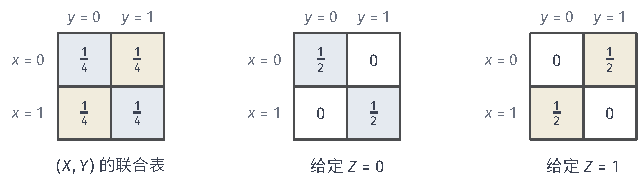
\includegraphics[width=108.6mm]{figures/07-probability/04-distribution-analysis/tikz/info-xor/figure.pdf}
  \caption{异或例子。左：独立公平硬币$(X,Y)$的联合表，蓝格$Z=X\oplus Y=0$，黄格$Z=1$。中、右：给定$Z=0$与$Z=1$后$(X,Y)$的条件表，质量只落在两格上，$Y$由$X$确定。}
  \label{fig:info-xor}
\end{BookInlineFigure}

图~\ref{fig:info-xor}给出了直观：单看$(X,Y)$，四格均匀，看不出任何关联；一旦知道$Z$，就只剩两格，$X$与$Y$紧紧绑在一起。$Z$本身不含关于$X$的信息，它提供的是$X$与$Y$之间的约束。

用链式法则从两个方向计算$I(X;Y,Z)$。先看$Y$再看$Z$：
\[
  I(X;Y)+I(X;Z\mid Y)=0+\ln2.
\]
先看$Z$再看$Y$：
\[
  I(X;Z)+I(X;Y\mid Z)=0+\ln2.
\]
两种顺序都给出$\ln2$：单独看$Y$或$Z$都毫无用处，两者合起来却完全确定$X$。

\paragraph{条件化可以减少互信息}
设$X$是公平硬币，$Y=Z=X$。则$I(X;Y)=H(X)=\ln2$；给定$Z$以后$X,Y$都已确定，$I(X;Y\mid Z)=0$。这次$Z$与$Y$携带的是同一份信息，知道$Z$以后，$Y$不再提供新东西。

两个例子放在一起说明，“三圈公共部分”$I(X;Y)-I(X;Y\mid Z)$在异或例子中等于$-\ln2$，在复制例子中等于$\ln2$。图~\ref{fig:info-venn}那样的记账图不能推广到三个变量的面积图，条件化前后的互信息要分别计算。


\section{交叉熵}
\label{sec:info-cross-entropy}

图~\ref{fig:info-question-tree}的提问方案是按真实概率$(\tfrac12,\tfrac14,\tfrac18,\tfrac18)$设计的：越常见的结果问得越少。如果设计者误以为四个字母等可能，就会给每个字母都安排两题；如果误以为概率是$(\tfrac18,\tfrac18,\tfrac14,\tfrac12)$，就会先问$d$、再问$c$，把最常见的$a$留到第三题。结果仍按真实分布出现，平均题数是多少，比按真实分布设计多出多少？

这类问题里有两个分布，角色不同。真实分布$P$决定结果出现的频率；参考分布$Q$决定给每个结果分配的代价$-\ln q(x)$，按$Q$看越常见的结果代价越小。平均代价按$P$计算。

\begin{definition}[交叉熵]
\label{def:info-cross-entropy}
设$P,Q$是可数集合$\mathcal{X}$上的概率分布，质量为$p,q$。$P$相对于参考分布$Q$的\term{交叉熵}（cross-entropy）是
\begin{equation}
  H(P,Q)=-\sum_{x\in\mathcal{X}}p(x)\ln q(x)=\mathbb{E}_{P}[-\ln q(X)]\in[0,+\infty],
  \label{eq:info-cross-entropy}
\end{equation}
约定$0\ln q=0$，而$p(x)>0$、$q(x)=0$的项为$+\infty$。若$P,Q$对同一参考测度（如Lebesgue测度）有密度$p,q$，在$\int p\lvert\ln q\rvert<\infty$时定义$H(P,Q)=-\int p\ln q$。
\end{definition}

$H(P,P)=H(P)$。离散时每一项$-p(x)\ln q(x)\geq0$，交叉熵总有意义。若真实分布给某个结果正概率，而参考分布给它零概率，这个结果的代价是无穷大，交叉熵也是无穷大：按参考分布设计的方案根本没有给它留位置。

\begin{theorem}[交叉熵的分解]
\label{thm:info-cross-entropy-decomposition}
设$P,Q$是可数集合上的概率分布，$H(P)<\infty$。则
\begin{equation}
  H(P,Q)=H(P)+D_{\mathrm{KL}}(P\Vert Q).
  \label{eq:info-cross-entropy-decomposition}
\end{equation}
所以$H(P,Q)\geq H(P)$，等号当且仅当$Q=P$。
\end{theorem}

\begin{proof}
若有$x$使$p(x)>0=q(x)$，则$P$不绝对连续于$Q$，两边都是$+\infty$。否则在$p(x)>0$的点，
\[
  -\ln q(x)=-\ln p(x)+\ln\frac{p(x)}{q(x)}.
\]
按$P$平均。第一项的期望是有限的$H(P)$，第二项的负部可积，期望是$D_{\mathrm{KL}}(P\Vert Q)\in[0,+\infty]$，所以期望可以拆开，得到式~\eqref{eq:info-cross-entropy-decomposition}。等号条件来自KL的零值条件。
\end{proof}

分解把平均代价分成两部分。$H(P)$是结果本身固有的不确定性，无论怎样设计都省不掉；$D_{\mathrm{KL}}(P\Vert Q)$是参考分布与真实分布不一致造成的额外代价。在所有参考分布中，交叉熵在$Q=P$时最小。若在一族参考分布中选使$H(P,Q)$最小的$Q$，由于$H(P)$不随$Q$改变，这等价于使$D_{\mathrm{KL}}(P\Vert Q)$最小；第~\ref{chap:distribution-approximation}章在一般分布族中研究这样的逼近。

\paragraph{四字母表的计算}
以bit为单位计算，此时$-\log_2q(x)$就是按$Q$设计的提问方案中$x$所需的题数。真实分布$P=(\tfrac12,\tfrac14,\tfrac18,\tfrac18)$，$H(P)=1.75$。取两个参考分布：
\[
  Q_1=(\tfrac14,\tfrac14,\tfrac14,\tfrac14),\qquad Q_2=(\tfrac18,\tfrac18,\tfrac14,\tfrac12).
\]
$Q_1$给每个字母$2$题，平均$2$题，所以$H(P,Q_1)=2$，$D_{\mathrm{KL}}(P\Vert Q_1)=0.25$。$Q_2$给$a,b,c,d$分别$3,3,2,1$题，平均
\[
  \tfrac12\cdot3+\tfrac14\cdot3+\tfrac18\cdot2+\tfrac18\cdot1=2.625,
\]
多付$0.875$题，这就是以bit计的$D_{\mathrm{KL}}(P\Vert Q_2)$。

\begin{BookInlineFigure}
  \centering
  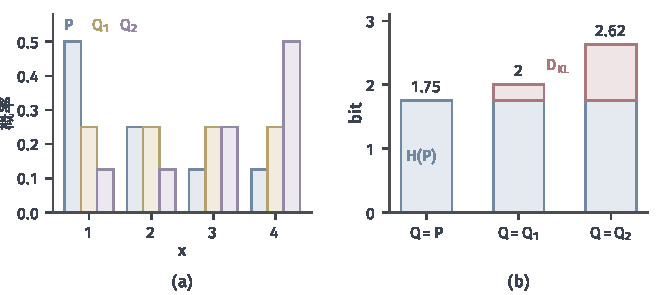
\includegraphics[width=112mm]{figures/07-probability/04-distribution-analysis/matplotlib/info-cross-entropy/figure.pdf}
  \caption{交叉熵的分解。(a)真实分布$P$（蓝）与两个参考分布$Q_1$（黄，均匀）、$Q_2$（紫）。(b)以bit计的$H(P,Q)$，蓝色部分是$H(P)=1.75$，红色部分是$D_{\mathrm{KL}}(P\Vert Q)$：$Q=P$时为$0$，$Q_1$时为$0.25$，$Q_2$时为$0.875$。}
  \label{fig:info-cross-entropy}
\end{BookInlineFigure}

图~\ref{fig:info-cross-entropy}显示，三种设计的蓝色部分一样高，差别全在红色部分。$Q_2$把最常见的结果当成最罕见的，失配最严重。

交叉熵的两个分布不能交换。真实分布为$Q_1$、参考分布为$P$时，四个字母等可能出现，而按$P$设计的题数是$1,2,3,3$，平均
\[
  H(Q_1,P)=\tfrac14(1+2+3+3)=2.25\neq H(P,Q_1)=2.
\]
两者的固有部分不同（$H(Q_1)=2$而$H(P)=1.75$），失配部分也不同（$0.25$与$0.25$恰好相等只是这个例子的巧合，一般不等）。若参考分布取$Q_3=(\tfrac12,\tfrac12,0,0)$，它完全没有为$c,d$留位置，$H(P,Q_3)=+\infty$。

\paragraph{熵为无穷时}
式~\eqref{eq:info-cross-entropy-decomposition}要求$H(P)<\infty$。若$H(P)=+\infty$，取$Q=P$，则$H(P,Q)=H(P)=+\infty$，而$D_{\mathrm{KL}}(P\Vert Q)=0$。这时“$D_{\mathrm{KL}}=H(P,Q)-H(P)$”是$\infty-\infty$，没有意义。KL散度直接由式~\eqref{eq:info-kl-recall}定义，不经过这个差。

\paragraph{连续情形}
对密度，交叉熵与微分熵一样依赖坐标。设$P=\mathcal{N}(0,1)$，$Q_s=\mathcal{N}(0,s^{2})$。参考分布分配的代价是
\[
  -\ln q_s(x)=\frac12\ln(2\pi s^{2})+\frac{x^{2}}{2s^{2}}.
\]
按$P$平均，用$\mathbb{E}_P[X^{2}]=1$，得到
\[
  H(P,Q_s)=\frac12\ln(2\pi s^{2})+\frac{1}{2s^{2}}.
\]
减去$h(P)=\tfrac12\ln(2\pi\mathrm{e})$，得到
\[
  D_{\mathrm{KL}}(P\Vert Q_s)=\ln s+\frac{1}{2s^{2}}-\frac12.
\]
$s=1$时为零；$s=2$时$H(P,Q_2)\approx1.737$，比$h(P)\approx1.419$多$0.318$。图~\ref{fig:info-gauss-cross}画出了整条曲线。

\begin{BookInlineFigure}
  \centering
  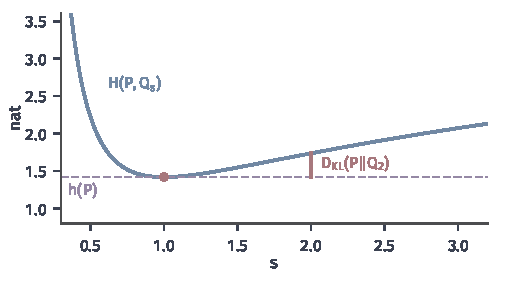
\includegraphics[width=86mm]{figures/07-probability/04-distribution-analysis/matplotlib/info-gauss-cross/figure.pdf}
  \caption{$P=\mathcal{N}(0,1)$相对于$Q_s=\mathcal{N}(0,s^{2})$的交叉熵（蓝），紫虚线为$h(P)\approx1.419$，单位nat。最小值在$s=1$（红点）处达到；红色竖线是$s=2$时的KL散度$0.318$。}
  \label{fig:info-gauss-cross}
\end{BookInlineFigure}

参考分布太窄（$s$小）时，交叉熵增长得很快：$P$的结果经常落在$Q_s$认为罕见的地方，每次都付很高的代价。太宽时增长较慢，只是对每个结果都略显“意外”。若把$x$换成$ax$，$h(P)$与$H(P,Q_s)$都增加$\ln\lvert a\rvert$，差$D_{\mathrm{KL}}$不变。连续情形下，有确定意义的是失配部分，而不是交叉熵本身的数值。

表~\ref{tab:info-entropy-cross}总结熵、交叉熵和KL散度的区别。

\begin{BookInlineTable}
  \centering
  \caption{熵、交叉熵与KL散度}
  \label{tab:info-entropy-cross}
  \begin{tabular}{@{}llll@{}}
    \toprule
    量 & 平均的对象 & 依赖坐标 & 下界\\
    \midrule
    $H(P)$或$h(P)$ & $P$下的$-\ln p$ & 连续时依赖 & 离散时$0$\\
    $H(P,Q)$ & $P$下的$-\ln q$ & 连续时依赖 & 离散时$H(P)$\\
    $D_{\mathrm{KL}}(P\Vert Q)$ & $P$下的$\ln(p/q)$ & 不依赖 & $0$\\
    \bottomrule
  \end{tabular}
\end{BookInlineTable}


\section{数据处理不等式}
\label{sec:info-data-processing}

观测$Y$含有关于$X$的信息$I(X;Y)$。实际中观测很少原样使用：读数会被四舍五入，记录会被压缩，信号会再经过一段有噪声的线路。处理后得到$Z$，它含有的关于$X$的信息能否比$Y$多？如果处理时只用了$Y$，没有再接触$X$的任何来源，答案应当是否定的。本节把“只用了$Y$”写成条件独立，再用互信息的链式法则证明这个直觉，并研究什么时候处理不损失信息。

\subsection{后处理的信息损失}
\label{sec:info-dpi-loss}

“$Z$只依赖$Y$”有两种说法。一种是生成方式：先有$(X,Y)$，再按一个只以$y$为输入的随机规则$K(y,\cdot)$产生$Z$，这个规则不看$X$。另一种是条件独立：$X\perp\!\!\!\perp Z\mid Y$。第~\ref{chap:conditional-distributions}章证明了两种说法在标准Borel空间上等价。满足这个条件时，称$X,Y,Z$构成\term{Markov链}（Markov chain），记作$X\to Y\to Z$。确定性处理$Z=g(Y)$是特例，规则$K(y,\cdot)$是点质量。

\begin{theorem}[数据处理不等式]
\label{thm:info-data-processing}
设$X,Y,Z$取值于标准Borel空间，$X\to Y\to Z$。则
\begin{equation}
  I(X;Z)\leq I(X;Y).
  \label{eq:info-data-processing}
\end{equation}
\end{theorem}

\begin{proof}
用链式法则~\eqref{eq:info-mi-chain-rule}按两种顺序展开$I(X;Y,Z)$。先$Y$后$Z$：
\[
  I(X;Y,Z)=I(X;Y)+I(X;Z\mid Y)=I(X;Y),
\]
其中$I(X;Z\mid Y)=0$由条件独立与定理~\ref{thm:info-conditional-mi-zero}得到。先$Z$后$Y$：
\[
  I(X;Y,Z)=I(X;Z)+I(X;Y\mid Z)\geq I(X;Z),
\]
因为条件互信息非负。两式合并即得式~\eqref{eq:info-data-processing}。整个论证只是非负量的相加和比较，在$[0,+\infty]$中进行，不需要任何熵有限。
\end{proof}

式~\eqref{eq:info-data-processing}称为\term{数据处理不等式}（data processing inequality）。证明还给出了损失的大小。若$I(X;Y)<\infty$，两种展开相等，移项得到
\begin{equation}
  I(X;Y)-I(X;Z)=I(X;Y\mid Z).
  \label{eq:info-dpi-gap}
\end{equation}
处理损失的信息，正是已知$Z$以后$Y$还能提供的关于$X$的信息。

\paragraph{两个例子}
图~\ref{fig:info-markov-chain}(a)是确定性的合并。$X$在$\{0,1,2,3\}$上均匀，$Y=X$，$Z=\lfloor Y/2\rfloor$把$0,1$并成$0$，把$2,3$并成$1$。由定理~\ref{thm:info-mi-entropy}，
\[
  I(X;Y)=H(X)=\ln4,\qquad I(X;Z)=H(Z)=\ln2.
\]
合并丢掉了“在组内是哪一个”这一位信息，损失$I(X;Y\mid Z)=\ln2$。

\begin{BookInlineFigure}
  \centering
  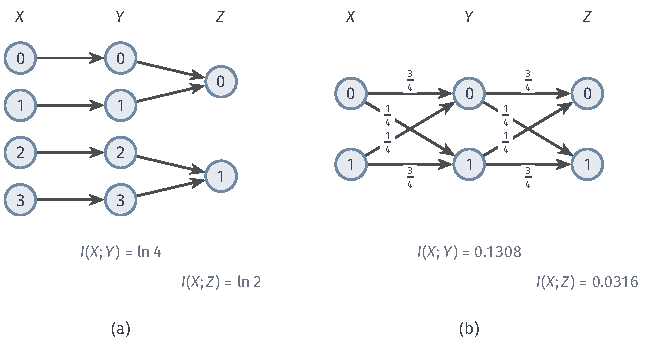
\includegraphics[width=110.1mm]{figures/07-probability/04-distribution-analysis/tikz/info-markov-chain/figure.pdf}
  \caption{两条Markov链$X\to Y\to Z$，箭头为转移概率。(a)$X$在四个标签上均匀，$Y=X$，$Z=\lfloor Y/2\rfloor$合并相邻标签。(b)公平硬币$X$经两段独立的线路，每段以概率$\tfrac14$翻转。下方为与$X$的互信息（nat）。}
  \label{fig:info-markov-chain}
\end{BookInlineFigure}

图~\ref{fig:info-markov-chain}(b)是添加独立噪声。$Y$是$X$经以概率$\tfrac14$出错的线路得到的，$Z$是$Y$再经一段独立的、以概率$\varepsilon_2$出错的线路得到的。$Z\neq X$当且仅当恰好一段出错，所以$X$到$Z$的总出错概率是
\[
  \tfrac14(1-\varepsilon_2)+\tfrac34\varepsilon_2.
\]
$\varepsilon_2=\tfrac14$时为$\tfrac38$，于是
\[
  I(X;Z)=\ln2-h_{\mathrm{b}}(\tfrac38)\approx0.0316<I(X;Y)\approx0.1308.
\]
图~\ref{fig:info-dpi-cascade}画出$I(X;Z)$随$\varepsilon_2$的变化：第二段线路越不可靠，剩下的信息越少，$\varepsilon_2=\tfrac12$时降为零。无论第二段怎样设计，曲线都不会越过$I(X;Y)$。

\begin{BookInlineFigure}
  \centering
  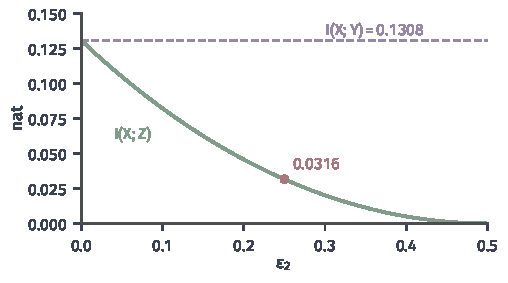
\includegraphics[width=86mm]{figures/07-probability/04-distribution-analysis/matplotlib/info-dpi-cascade/figure.pdf}
  \caption{两段串联线路。第一段翻转概率$\tfrac14$，第二段为$\varepsilon_2$。绿线为$I(X;Z)$，紫虚线为$I(X;Y)\approx0.1308$，单位nat；红点为$\varepsilon_2=\tfrac14$时的$0.0316$。}
  \label{fig:info-dpi-cascade}
\end{BookInlineFigure}

\paragraph{两个推论}
取$Z=g(Y)$为任意可测函数，得到$I(X;g(Y))\leq I(X;Y)$：任何对观测的计算都不能增加关于$X$的信息。再取离散的$X$并令$Y=X$，联合质量$p_{X,g(X)}(x,g(x))=p_X(x)$，代入式~\eqref{eq:info-mutual-information-discrete}，比值是$1/p_{g(X)}(g(x))$，所以$I(X;g(X))=H(g(X))$，特别地$I(X;X)=H(X)$。于是
\[
  H(g(X))\leq H(X).
\]
对离散变量作函数变换只会合并取值，熵不增；$g$是单射时取等号。注意微分熵没有这个性质，式~\eqref{eq:info-differential-entropy-scale}中$\lvert a\rvert>1$时$h(aX)>h(X)$。

\paragraph{条件独立的作用}
定理的前提不能去掉。仍看图~\ref{fig:info-markov-chain}(b)的第一段：$Y=X\oplus N$，$N$是翻转噪声。若处理者碰巧知道$N$，令$Z=Y\oplus N$，则$Z=X$，$I(X;Z)=\ln2$，远大于$I(X;Y)$。这里$Z$不只依赖$Y$，还依赖与$X$在给定$Y$时相关的$N$：给定$Y=y$时，$N=0$当且仅当$X=y$。所以$X\perp\!\!\!\perp Z\mid Y$不成立。“只用了$Y$”的确切意思是：处理中引入的额外随机性，在给定$Y$时与$X$独立。

条件独立是对称的：$X\perp\!\!\!\perp Z\mid Y$等价于$Z\perp\!\!\!\perp X\mid Y$，所以$X\to Y\to Z$也是$Z\to Y\to X$，同样有$I(X;Z)\leq I(Y;Z)$。箭头只是书写习惯。Markov链描述的是联合分布的一种结构，信息在其中两端都要经过$Y$；它并不规定哪个变量产生了哪个变量。同一个联合分布既可以由“$X$经过线路得到$Y$”产生，也可以由“先抽$Y$、再按后验抽$X$”产生，不等式对两者相同。

\subsection{信息保留}
\label{sec:info-dpi-preservation}

数据处理不等式什么时候取等号？最简单的情形是处理可以撤销。设$Z=g(Y)$，其中$g$是可测双射，逆映射也可测。则$X\to Y\to Z$，同时$Y=g^{-1}(Z)$，又有$X\to Z\to Y$。对两条链分别应用定理~\ref{thm:info-data-processing}，得到
\[
  I(X;Z)\leq I(X;Y)\leq I(X;Z),
\]
所以$I(X;g(Y))=I(X;Y)$。对两个变量分别作这样的变换，互信息都不变；这与微分熵随坐标改变形成对比。

可逆是充分条件，不是必要条件。设$X$是公平硬币，$U$是与$X$独立的公平硬币，观测$Y=2X+U\in\{0,1,2,3\}$，处理为$Z=\lfloor Y/2\rfloor$。$Z=X$，所以
\[
  I(X;Z)=H(X)=\ln2.
\]
另一方面，$X$是$Y$的函数，$I(X;Y)=H(X)-H(X\mid Y)=\ln2$。处理把四个值并成两个，不可逆，却没有损失任何关于$X$的信息：被丢掉的$U$与$X$无关。

一般的判据由式~\eqref{eq:info-dpi-gap}给出。

\begin{theorem}[信息保留的条件]
\label{thm:info-dpi-equality}
设$X,Y,Z$取值于标准Borel空间，$X\to Y\to Z$，并且$I(X;Y)<\infty$。则$I(X;Z)=I(X;Y)$当且仅当$X\perp\!\!\!\perp Y\mid Z$，即$X\to Z\to Y$也成立。
\end{theorem}

\begin{proof}
由式~\eqref{eq:info-dpi-gap}，等号当且仅当$I(X;Y\mid Z)=0$，再由定理~\ref{thm:info-conditional-mi-zero}，这等价于$X\perp\!\!\!\perp Y\mid Z$。
\end{proof}

$X\to Z\to Y$说的是：知道$Z$以后，$Y$中剩下的部分与$X$无关。上面的例子中，给定$Z=X$以后，$Y$只多出一个独立的$U$，确实与$X$条件独立。在图~\ref{fig:info-markov-chain}(a)中，给定$Z=0$时$Y$在$\{0,1\}$中仍随$X$变化，条件独立不成立，信息有损失。

定理要求$I(X;Y)<\infty$，因为式~\eqref{eq:info-dpi-gap}要移项。互信息为无穷时，$I(X;Z)=I(X;Y)=\infty$可以与“有损失”同时出现。设$X\sim\operatorname{Unif}(0,1)$，$Y=X$，$Z$由$X$二进制展开的奇数位组成。$Z$本身服从无原子的分布，并且是$X$的函数，与第~\ref{sec:info-mi-definition}节的对角线论证相同，联合分布集中在一个函数图像上，而边缘乘积给这个图像零概率，所以$I(X;Z)=+\infty=I(X;Y)$。但给定$Z$以后，$X$的偶数位仍是独立均匀的，$Y=X$与$X$之间还有无穷多的信息，$I(X;Y\mid Z)=+\infty$。两边都是无穷，比较互信息的数值已经看不出损失，要直接看条件互信息。


\section{辨别错误的下界}
\label{sec:info-fano}

一个标签$X$取$M$个值之一，我们只能看到与它相关的观测$Y$，要根据$Y$猜出$X$。无论怎样设计判别规则，错误概率能否降到任意小？直觉上，若看到$Y$以后$X$仍然很不确定，就不可能总猜对。本节把这个直觉定量化：剩余的不确定性$H(X\mid Y)$给错误概率一个下界。随后把它改写为互信息的形式，这是证明“信息不够时无法可靠辨别”的通用工具。

\subsection{Fano不等式}
\label{sec:info-fano-inequality}

先固定设定。$X$取值于$M\geq2$个元素的有限集合$\mathcal{X}$；观测$Y$取值于标准Borel空间，可以是离散的，也可以是连续的。判别规则是可测函数$g$，猜测$\hat{X}=g(Y)\in\mathcal{X}$，错误概率$P_{\mathrm{e}}=\mathbb{P}(\hat{X}\neq X)$。

$Y$不一定离散，所以条件熵按正则条件分布逐个$y$定义：
\[
  H(X\mid Y)=\int H\bigl(P_{X\mid Y}(\cdot\mid y)\bigr)\,P_Y(\mathrm{d}y),
\]
其中$H(\cdot)$是有限概率表的熵。$Y$离散时它就是式~\eqref{eq:info-conditional-entropy}。

\begin{theorem}[Fano不等式]
\label{thm:info-fano}
在上述设定下，
\begin{equation}
  H(X\mid Y)\leq h_{\mathrm{b}}(P_{\mathrm{e}})+P_{\mathrm{e}}\ln(M-1).
  \label{eq:info-fano}
\end{equation}
\end{theorem}

式~\eqref{eq:info-fano}称为\term{Fano不等式}（Fano's inequality）。证明的想法是引入错误指示$E=\mathbf{1}_{\{\hat{X}\neq X\}}$，把“确定$X$”拆成两步：先确定是否猜错，再在猜错时确定$X$是其余$M-1$个值中的哪一个。第一步最多需要$h_{\mathrm{b}}(P_{\mathrm{e}})$，第二步只在猜错时才需要，最多$\ln(M-1)$。

\begin{proof}
固定$y$，在条件分布$P_{X\mid Y}(\cdot\mid y)$下考虑离散变量$X$与$E=\mathbf{1}_{\{g(y)\neq X\}}$。$E$是$X$的函数，所以$(X,E)$与$X$的概率表只差零概率的格，二者熵相等。对$(E,X)$用链式法则，先揭示$E$：
\[
  H(X\mid Y=y)=H(E\mid Y=y)+H(X\mid E,Y=y).
\]
记$e(y)=\mathbb{P}(X\neq g(y)\mid Y=y)$。第一项是$h_{\mathrm{b}}(e(y))$。第二项中，$E=0$时$X=g(y)$已确定，熵为$0$；$E=1$时$X$在$\mathcal{X}\setminus\{g(y)\}$的$M-1$个值中，由定理~\ref{thm:info-entropy-range}熵至多$\ln(M-1)$。所以
\[
  H(X\mid Y=y)\leq h_{\mathrm{b}}(e(y))+e(y)\ln(M-1).
\]
对$P_Y$积分，$\int e(y)\,P_Y(\mathrm{d}y)=P_{\mathrm{e}}$。$h_{\mathrm{b}}$凹，由Jensen不等式，
\[
  \int h_{\mathrm{b}}(e(y))\,P_Y(\mathrm{d}y)\leq h_{\mathrm{b}}(P_{\mathrm{e}}).
\]
两部分合起来即得式~\eqref{eq:info-fano}。
\end{proof}

若判别时还使用了与$(X,Y)$独立的随机数$U$，把$(Y,U)$看成观测即可：$U$与$(X,Y)$独立，所以给定$(Y,U)$时$X$的条件分布与给定$Y$时相同，$H(X\mid Y,U)=H(X\mid Y)$，定理不变。

\paragraph{怎样读这个不等式}
记右端为$\phi_M(p)=h_{\mathrm{b}}(p)+p\ln(M-1)$。求导得$\phi_M'(p)=\ln\frac{(1-p)(M-1)}{p}$，在$p<(M-1)/M$时为正，所以$\phi_M$在$[0,(M-1)/M]$上严格递增，从$0$升到$\phi_M((M-1)/M)=\ln M$。于是，若$H(X\mid Y)=c>0$，任何规则的错误概率都不小于方程$\phi_M(p)=c$在这段区间上的解。剩余不确定性越大，错误下界越高；$H(X\mid Y)=0$时下界为零，与$X$可由$Y$确定一致。

由$h_{\mathrm{b}}(p)\leq\ln2$，可以得到一个便于计算的较弱形式：$M\geq3$时，
\begin{equation}
  P_{\mathrm{e}}\geq\frac{H(X\mid Y)-\ln2}{\ln(M-1)}.
  \label{eq:info-fano-weak}
\end{equation}
它在$H(X\mid Y)\leq\ln2$时没有用处，在标签很多时与精确形式相差不大。

\paragraph{等号可以达到}
设$M=4$，$X$在$\{1,2,3,4\}$上均匀；观测$Y$以概率$0.7$等于$X$，以概率$0.1$等于其余三个值中的每一个。由对称性，给定$Y=y$时，$X=y$的后验概率是$0.7$，其余三个值各$0.1$。于是
\[
  H(X\mid Y)=H(0.7,0.1,0.1,0.1)=h_{\mathrm{b}}(0.3)+0.3\ln3\approx0.940\ \mathrm{nat}.
\]
猜$\hat{X}=Y$的错误概率是$0.3$，代入式~\eqref{eq:info-fano}右端恰好也是$0.940$：等号成立。由$\phi_4$的单调性，任何规则的错误概率都至少是$0.3$，所以猜$\hat{X}=Y$已是最好的规则。

\begin{BookInlineFigure}
  \centering
  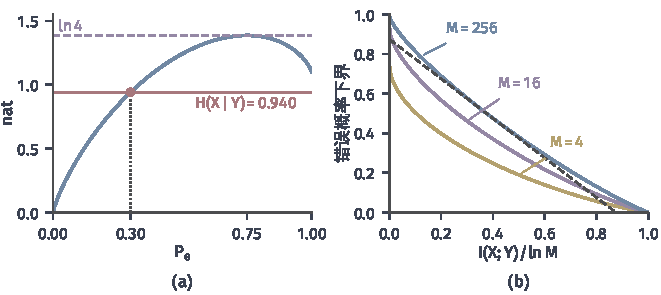
\includegraphics[width=112mm]{figures/07-probability/04-distribution-analysis/matplotlib/info-fano/figure.pdf}
  \caption{Fano不等式。(a)$M=4$时$\phi_4(P_{\mathrm{e}})=h_{\mathrm{b}}(P_{\mathrm{e}})+P_{\mathrm{e}}\ln3$（蓝），在$P_{\mathrm{e}}=\tfrac34$处达到$\ln4$（紫虚线）。红线为四值对称观测例子的$H(X\mid Y)\approx0.940$，与曲线交于$P_{\mathrm{e}}=0.3$。(b)$X$均匀时Fano给出的最小错误概率，横轴为$I(X;Y)/\ln M$，$M=4,16,256$；灰虚线为$M=256$时式~\eqref{eq:info-fano-mi}的较弱形式。}
  \label{fig:info-fano}
\end{BookInlineFigure}

等号成立的条件从证明中可以读出：每个$y$下错误概率相同（Jensen取等），并且猜错时其余$M-1$个值等可能。上面的例子两条都满足。一般情形下Fano不等式只是下界，实际最小错误可以大得多。

定理只适用于有限个标签和“猜错与否”这种错误标准。若要估计的是连续参数，“猜中”的概率通常为零，不等式不能直接使用；需要先从参数中挑出有限个相互分开的候选，把估计问题改写成在它们之间辨别，下一小节会看到这种改写的样子。

\subsection{通信与统计辨别}
\label{sec:info-fano-applications}

当$X$在$M$个标签上均匀时，$H(X)=\ln M$，由式~\eqref{eq:info-mi-entropy-difference}，$H(X\mid Y)=\ln M-I(X;Y)$。这里$Y$可以不是离散的，第~\ref{sec:info-mi-entropy}节的证明逐个条件值进行，同样成立。代入较弱形式（这次用$\ln M$代替$\ln(M-1)$，对$M=2$也适用），得到
\begin{equation}
  P_{\mathrm{e}}\geq1-\frac{I(X;Y)+\ln2}{\ln M}.
  \label{eq:info-fano-mi}
\end{equation}
这个形式只需要互信息：要以小错误区分$M$个等可能的标签，观测至少要提供约$\ln M$的信息。四值对称观测的例子中$I(X;Y)=\ln4-0.940\approx0.446$，式~\eqref{eq:info-fano-mi}给出$P_{\mathrm{e}}\geq0.178$，比精确形式的$0.3$弱。图~\ref{fig:info-fano}(b)比较了不同$M$时的精确下界：横轴按$\ln M$归一化后，$M$越大，曲线越接近直线$1-I/\ln M$。

\paragraph{通信}
在有噪声的线路上传送消息时，消息$W$从$M$个中均匀选出，编码成线路输入$X_1,\dots,X_n$，线路输出$Y_1,\dots,Y_n$，接收方据此猜出$\hat{W}$。码率$R=\ln M/n$是每次使用线路平均传送的信息。由于$\hat{W}$只依赖输出，$W\to(Y_1,\dots,Y_n)\to\hat{W}$；由于输出只经由输入依赖消息，数据处理不等式给出
\[
  I(W;Y_1,\dots,Y_n)\leq I(X_1,\dots,X_n;Y_1,\dots,Y_n).
\]
第~\ref{chap:discrete-channel-capacity}章会证明，对每次使用相互独立的线路，右端不超过$nC$，$C$是单次使用的容量。代入式~\eqref{eq:info-fano-mi}，得到
\[
  P_{\mathrm{e}}\geq1-\frac{nC+\ln2}{nR}=1-\frac{C}{R}-\frac{\ln2}{nR}.
\]
若$R>C$，$n\to\infty$时右端趋于$1-C/R>0$，错误概率不能趋于零。这里的错误概率是按均匀消息平均的；逐个消息的最大错误概率不小于平均值，下界对它同样成立。

\paragraph{统计辨别}
设有$M$个候选分布$P_1,\dots,P_M$，标签$J$均匀选出，观测是来自$P_J$的独立同分布样本$X_1,\dots,X_n$，要从样本猜出$J$。这时需要的是$I(J;X_1,\dots,X_n)$的上界。

离散情形下，对任意分布$Q$，记$\bar{P}=\tfrac1M\sum_jP_j$为观测的边缘分布，在各项有限时直接展开对数可以核对
\[
  \frac1M\sum_{j=1}^{M}D_{\mathrm{KL}}(P_j\Vert Q)=I(J;X)+D_{\mathrm{KL}}(\bar{P}\Vert Q),
\]
依据是对数比的拆分
\[
  \ln\frac{p_j(x)}{q(x)}=\ln\frac{p_j(x)}{\bar{p}(x)}+\ln\frac{\bar{p}(x)}{q(x)}.
\]
按权重$\tfrac1Mp_j(x)$对$j$与$x$求和，第一项给出$I(J;X)$（$(J,X)$的联合质量是$\tfrac1Mp_j(x)$，边缘乘积是$\tfrac1M\bar{p}(x)$），第二项给出$D_{\mathrm{KL}}(\bar{P}\Vert Q)$。右端第二项非负，所以
\[
  I(J;X)\leq\frac1M\sum_{j=1}^{M}D_{\mathrm{KL}}(P_j\Vert Q).
\]
取$Q$为某个候选$P_k$，就得到$I(J;X)\leq\max_{j,k}D_{\mathrm{KL}}(P_j\Vert P_k)$。$n$个独立样本时，乘积分布的对数比是各样本对数比之和，KL随之乘以$n$。于是
\[
  P_{\mathrm{e}}\geq1-\frac{n\max_{j,k}D_{\mathrm{KL}}(P_j\Vert P_k)+\ln2}{\ln M}.
\]

例如$M=8$个候选$\mathcal{N}(\theta_j,1)$，$\theta_j=0,0.1,\dots,0.7$。按定义计算，
\[
  D_{\mathrm{KL}}\bigl(\mathcal{N}(a,1)\Vert\mathcal{N}(b,1)\bigr)=\mathbb{E}\Bigl[\frac{(X-b)^{2}-(X-a)^{2}}{2}\Bigr]=\frac{(a-b)^{2}}{2},
\]
期望对$X\sim\mathcal{N}(a,1)$取。最大值是$0.7^{2}/2=0.245$，一个样本时$P_{\mathrm{e}}\geq1-(0.245+\ln2)/\ln8\approx0.549$。候选越密、样本越少，辨别越难；要让下界失效，样本数须与$\ln M/\max D_{\mathrm{KL}}$同阶。

这两个应用用的是同一个工具，但要分别核对三件事：标签是否均匀（Fano给的是平均错误）、观测是怎样由标签产生的（决定互信息的上界）、错误按什么标准计算。把估计连续参数的误差转成在候选之间的辨别错误，是卷八的工作，可参考\BookChapterRef{chap:finite-sample-lower-bounds}{卷八第5章“有限样本的精度下界”}。


\section{互信息的辨别下界}
\label{sec:info-infonce}

上一节用互信息的上界推出辨别错误的下界。这一节方向相反：互信息本身难以计算时，用一个辨别问题做得有多好，给出互信息的下界。

互信息需要联合分布与边缘乘积的密度比$r=\mathrm{d}P_{X,Y}/\mathrm{d}(P_X\otimes P_Y)$，再对它取对数积分。在高维连续空间里，$r$常常写不出来，积分也难以计算；但从$P_{X,Y}$抽取配对$(X,Y)$、从$P_Y$抽取单个$Y$往往很容易。于是考虑一个辅助问题：把一个真正与$X$配对的$Y$藏在一堆与$X$无关的候选中，让一个评分规则把它找出来。$X$与$Y$关联越强，真配对越容易被认出；找得好，就说明互信息至少有这么大。

\subsection{候选配对的构造}
\label{sec:info-infonce-construction}

设$X,Y$取值于标准Borel空间，联合分布$P_{X,Y}$，正则条件分布$P_{Y\mid X}$存在。固定候选数$N\geq2$，按下面的方式产生$(X,J,Y_1,\dots,Y_N)$：
\begin{enumerate}
  \item 抽取$X\sim P_X$，并独立地从$\{1,\dots,N\}$中均匀抽取隐藏位置$J$；
  \item 给定$X=x$、$J=j$，令$Y_j\sim P_{Y\mid X}(\cdot\mid x)$，其余$Y_k\sim P_Y$（$k\neq j$），这$N$个候选在给定$(X,J)$时相互独立。
\end{enumerate}
记观测为$W=(X,Y_1,\dots,Y_N)$，$J$不被观测。图~\ref{fig:info-infonce-construction}画出了$N=4$时的构造。

\begin{BookInlineFigure}
  \centering
  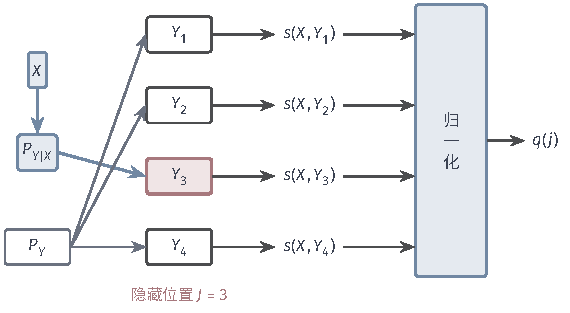
\includegraphics[width=96.4mm]{figures/07-probability/04-distribution-analysis/tikz/info-infonce-construction/figure.pdf}
  \caption{$N=4$个候选的构造。隐藏位置$J=3$（红框）的候选按给定$X$的条件分布$P_{Y\mid X}$产生（蓝），其余候选独立地按边缘分布$P_Y$产生（灰）。评分$s(X,Y_j)$经指数归一化得到对隐藏位置的猜测$q(j)$。}
  \label{fig:info-infonce-construction}
\end{BookInlineFigure}

这个构造有三条基本性质，后面的证明都靠它们。

\begin{lemma}[候选的分布]
\label{lem:info-infonce-structure}
在上述构造中：
\begin{enumerate}
  \item $J$与$X$独立；
  \item $(Y_1,\dots,Y_N)$独立同分布于$P_Y$，并且与$J$独立；
  \item 给定$J=j$，$(X,Y_j)$的分布是$P_{X,Y}$，其余候选独立同分布于$P_Y$，并与$(X,Y_j)$独立。
\end{enumerate}
\end{lemma}

\begin{proof}
第一条是构造的第一步。第三条：给定$J=j$，$X\sim P_X$且$Y_j$按$P_{Y\mid X}$产生，所以$(X,Y_j)\sim P_{X,Y}$；其余候选的条件分布不依赖$X$，所以与$(X,Y_j)$独立。第二条：在第三条中对$X$积分，$Y_j$的分布是$P_Y$，其余候选也是$P_Y$，且相互独立；这个分布不依赖$j$，所以候选组与$J$独立。
\end{proof}

第二条说明，单看候选组而不看$X$，完全看不出哪个是真配对；隐藏位置的线索只能来自$X$与各候选之间的关联。

\paragraph{隐藏位置的后验}
设$P_{X,Y}\ll P_X\otimes P_Y$，密度比为$r(x,y)$；$I(X;Y)<\infty$时这总成立。由引理~\ref{lem:info-infonce-structure}第三条，给定$J=j$时$W$的分布是$P_{X,Y_j}\otimes P_Y^{\otimes(N-1)}$，它相对于参考分布$P_X\otimes P_Y^{\otimes N}$的密度是$r(x,y_j)$。$J$的先验是$1/N$，由Bayes公式，
\begin{equation}
  \mathbb{P}(J=j\mid W)=\frac{r(X,Y_j)}{\sum_{k=1}^{N}r(X,Y_k)},\qquad j=1,\dots,N.
  \label{eq:info-infonce-posterior}
\end{equation}
分母几乎必然为正，因为真配对一项$r(X,Y_J)$几乎必然为正。后验只依赖各候选的密度比：与$X$越“般配”的候选，越可能是真配对。$X$与$Y$独立时$r\equiv1$，后验是均匀分布，候选无从区分。

\paragraph{二元例子}
仍用公平硬币$X$经以概率$\tfrac14$出错的线路得到$Y$。密度比在$y=x$时为$\tfrac{3/8}{1/4}=\tfrac32$，在$y\neq x$时为$\tfrac12$。取$N=2$。若两个候选相同（都等于$X$或都不等于$X$），后验是$(\tfrac12,\tfrac12)$；若只有一个等于$X$，由式~\eqref{eq:info-infonce-posterior}，它是真配对的后验概率为
\[
  \frac{3/2}{3/2+1/2}=\frac34.
\]
真配对等于$X$的概率是$\tfrac34$，另一个候选与$X$无关、是公平硬币，所以两个候选不同的概率恰为$\tfrac12$。

\subsection{InfoNCE下界}
\label{sec:info-infonce-bound}

实际中密度比$r$未知，用一个可测的实值\term{配对评分}（critic）函数$s(x,y)$代替$\ln r$，把评分作指数归一化得到对隐藏位置的猜测：
\begin{equation}
  q_s(j\mid W)=\frac{\mathrm{e}^{s(X,Y_j)}}{\sum_{k=1}^{N}\mathrm{e}^{s(X,Y_k)}}.
  \label{eq:info-infonce-softmax}
\end{equation}
用真实位置的平均负对数概率衡量猜得好坏，
\begin{equation}
  L(s)=\mathbb{E}\bigl[-\ln q_s(J\mid W)\bigr]\in[0,+\infty].
  \label{eq:info-infonce-loss}
\end{equation}
$L(s)$是真实后验相对于猜测$q_s$的交叉熵按$W$的平均。以$L$为目标的方法通称InfoNCE（信息噪声对比估计），它的总体值给出互信息的下界。

\begin{theorem}[InfoNCE下界]
\label{thm:info-infonce}
设$X,Y$取值于标准Borel空间，$I(X;Y)<\infty$，$N\geq2$，$s$是任意可测实值评分函数。则
\begin{equation}
  \ln N-L(s)\leq I(X;Y).
  \label{eq:info-infonce-bound}
\end{equation}
更精确地，
\begin{equation}
  I(X;Y)-\bigl(\ln N-L(s)\bigr)=I(X;Y_1,\dots,Y_N)+\mathbb{E}\Bigl[D_{\mathrm{KL}}\bigl(P_{J\mid W}\Vert q_s(\cdot\mid W)\bigr)\Bigr].
  \label{eq:info-infonce-gap}
\end{equation}
\end{theorem}

证明分三步：猜测的交叉熵不小于后验的熵；后验的熵等于$\ln N$减去隐藏位置与观测的互信息；这个互信息不超过原配对的互信息。

\begin{proof}
\emph{第一步。}固定$W=w$，$J$的后验$\pi(\cdot\mid w)$是$N$个点上的概率表。由定理~\ref{thm:info-cross-entropy-decomposition}（$N$点上的熵有限），
\[
  \mathbb{E}\bigl[-\ln q_s(J\mid W)\bigm|W=w\bigr]=H\bigl(\pi(\cdot\mid w)\bigr)+D_{\mathrm{KL}}\bigl(\pi(\cdot\mid w)\Vert q_s(\cdot\mid w)\bigr).
\]
对$W$平均，左端是$L(s)$，右端第一项是$H(J\mid W)$，于是
\[
  L(s)=H(J\mid W)+\mathbb{E}\bigl[D_{\mathrm{KL}}(P_{J\mid W}\Vert q_s(\cdot\mid W))\bigr]\geq H(J\mid W).
\]

\emph{第二步。}$J$均匀，$H(J)=\ln N$有限，由式~\eqref{eq:info-mi-entropy-difference}（对一般的$W$逐条件值进行），
\[
  H(J\mid W)=\ln N-I(J;W).
\]

\emph{第三步。}记$\bm{Y}=(Y_1,\dots,Y_N)$。用链式法则~\eqref{eq:info-mi-chain-rule}展开$I(J;W)=I(J;\bm{Y},X)$，由引理第二条$I(J;\bm{Y})=0$，所以
\[
  I(J;W)=I(J;X\mid\bm{Y}).
\]
另一方面，用两种顺序展开$I(X;J,\bm{Y})$。先$J$后$\bm{Y}$：由引理第一条$I(X;J)=0$；由引理第三条，给定$J=j$时只有$Y_j$与$X$相关，再用一次链式法则得$I(X;\bm{Y}\mid J)=I(X;Y)$。于是
\[
  I(X;J,\bm{Y})=I(X;Y).
\]
先$\bm{Y}$后$J$：
\[
  I(X;J,\bm{Y})=I(X;\bm{Y})+I(X;J\mid\bm{Y}).
\]
两式相等，而$I(X;Y)<\infty$，所以各项有限，可以移项，并由条件互信息的对称性得到
\[
  I(J;W)=I(X;J\mid\bm{Y})=I(X;Y)-I(X;\bm{Y}).
\]

三步合起来，
\[
  \ln N-L(s)=I(X;Y)-I(X;\bm{Y})-\mathbb{E}\bigl[D_{\mathrm{KL}}(P_{J\mid W}\Vert q_s)\bigr].
\]
这就是式~\eqref{eq:info-infonce-gap}；右端两个减项都非负，得到式~\eqref{eq:info-infonce-bound}。若$L(s)=+\infty$，式~\eqref{eq:info-infonce-bound}左端为$-\infty$，自然成立。
\end{proof}

式~\eqref{eq:info-infonce-gap}说明下界与真值之间有两段差距。第二段来自评分函数：只有$q_s$等于真实后验时才消失，由式~\eqref{eq:info-infonce-posterior}，这要求$s(x,y)=\ln r(x,y)+c(x)$，其中$c(x)$只依赖$x$（它在归一化中相消）。第一段$I(X;\bm{Y})$与评分无关，是辅助问题本身的损失：$X$与整组候选的互信息。它非负，所以即使评分最优，下界一般也严格小于$I(X;Y)$。

\paragraph{二元例子的计算}
取最优评分$s=\ln r$。$N=2$时，上一小节已得到：以概率$\tfrac12$两个候选相同，后验熵为$\ln2$；以概率$\tfrac12$两者不同，后验为$(\tfrac34,\tfrac14)$，熵为$h_{\mathrm{b}}(\tfrac14)$。于是
\[
  H(J\mid W)=\tfrac12\ln2+\tfrac12h_{\mathrm{b}}(\tfrac14)\approx0.3466+0.2812=0.6277.
\]
下界为
\[
  \ln2-L(\ln r)=\ln2-H(J\mid W)\approx0.0654,
\]
恰为$I(X;Y)\approx0.1308$的一半；由式~\eqref{eq:info-infonce-gap}，另一半是$I(X;\bm{Y})$。候选数增加时，计算方法相同：给定$X$，真配对以概率$\tfrac34$与$X$相同，其余$N-1$个候选各以概率$\tfrac12$与$X$相同，按相同候选的个数$m$求和，后验在相同者上为$\tfrac{3/2}{Z}$、在其余者上为$\tfrac{1/2}{Z}$，$Z=\tfrac32m+\tfrac12(N-m)$。

\begin{BookInlineFigure}
  \centering
  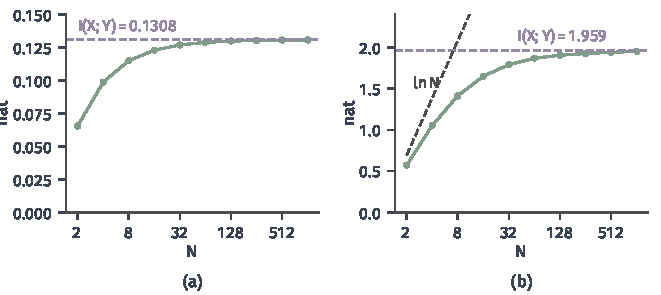
\includegraphics[width=112mm]{figures/07-probability/04-distribution-analysis/matplotlib/info-infonce-bound/figure.pdf}
  \caption{最优评分下的InfoNCE下界$\ln N-L$（绿）随候选数$N$的变化，横轴为对数刻度，紫虚线为$I(X;Y)$。(a)二元例子，按相同候选个数精确求和：$N=2,4,16,1024$时为$0.0654,0.0987,0.1229,0.1307$。(b)相关系数$0.99$的二元标准正态，$I(X;Y)\approx1.959$；Monte Carlo估计，种子$0$，每个$N$用$40000$组样本，标准误不超过$0.005$；灰虚线为$\ln N$。}
  \label{fig:info-infonce-bound}
\end{BookInlineFigure}

图~\ref{fig:info-infonce-bound}(a)中，下界随$N$增加逐渐逼近$I(X;Y)$：候选越多，$X$与整组候选的互信息在总量中所占的份额越小。这与“多个干扰项中认出真配对”的直觉一致，干扰项越多，认出真配对越能说明关联强。

\subsection{下界的限制}
\label{sec:info-infonce-limits}

\paragraph{候选数的上限}
$q_s\leq1$，所以$L(s)\geq0$，从而
\[
  \ln N-L(s)\leq\ln N.
\]
无论评分多好，下界都不超过$\ln N$。$I(X;Y)$很大时，要让下界接近它，候选数须达到$\mathrm{e}^{I(X;Y)}$的量级。图~\ref{fig:info-infonce-bound}(b)中相关系数为$0.99$的正态配对，$I(X;Y)\approx1.959$，$\mathrm{e}^{1.959}\approx7.1$；$N=2$时下界只有$0.57$，比$\ln2$略小，$N=8$时约$1.41$，直到$N$达到数百才接近真值。互信息每增加$1$ nat，所需候选数约乘以$\mathrm{e}$。

\paragraph{评分函数的限制}
评分函数通常只能从一个给定的函数类中选。在二元例子中限定$s(x,y)=c\,\mathbf{1}_{\{x=y\}}$，只调一个参数$c$。$N=2$时可以逐项算出$\ln2-L$：两个候选相同时$q$均匀；不同时真配对与$X$相同的概率是$\tfrac34$，被赋予$\mathrm{e}^{c}/(\mathrm{e}^{c}+1)$。于是
\[
  L(c)=\tfrac12\ln2+\tfrac12\Bigl[\tfrac34\ln(1+\mathrm{e}^{-c})+\tfrac14\ln(1+\mathrm{e}^{c})\Bigr].
\]
令导数为零得$\mathrm{e}^{c}=3$，$c=\ln3$正是$\ln\tfrac32-\ln\tfrac12$，这时评分等于$\ln r$加常数，下界达到$0.0654$。

\begin{BookInlineFigure}
  \centering
  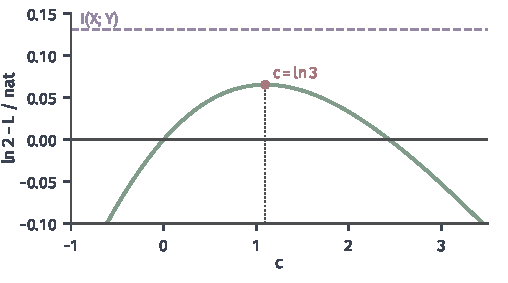
\includegraphics[width=86mm]{figures/07-probability/04-distribution-analysis/matplotlib/info-infonce-score/figure.pdf}
  \caption{二元例子、$N=2$、评分限定为$s(x,y)=c\,\mathbf{1}_{\{x=y\}}$时的$\ln2-L$（绿），紫虚线为$I(X;Y)\approx0.1308$。最大值在$c=\ln3$（红点）处，为$0.0654$；$c=0$时为$0$，$c=3$时约为$-0.053$。}
  \label{fig:info-infonce-score}
\end{BookInlineFigure}

图~\ref{fig:info-infonce-score}显示，$c=0$时评分不区分候选，下界为零；$c$过大时评分过于自信，猜错的代价很高，“下界”变成负数，仍然正确却毫无用处。一般的函数类不一定包含$\ln r+c(x)$，最优的$s$也只能逼近，式~\eqref{eq:info-infonce-gap}中的第二段差距一般不为零。

\paragraph{下界小不能推出独立}
由于上面两段差距，$\ln N-L(s)$接近零可能只是因为$N$太小、评分函数类太窄或选得不好。下界为零与$I(X;Y)=0$不是一回事；InfoNCE不是判断独立的判据，只是在已知互信息存在、需要其数值大小时提供的可计算下界。比较各种依赖度量能否刻画独立，是第~\ref{chap:dependence-measures}章的问题。

\paragraph{总体值与样本值}
定理~\ref{thm:info-infonce}中的$L(s)$是总体期望。实际计算时用一批样本的平均代替它，并且常用同一批样本挑选评分函数。样本平均有随机误差，可能高于真实的$L(s)$，也可能低于它；在同一批样本上挑出的评分，其样本平均系统性地偏低。所以单批样本得到的经验值并不自动是互信息的下界，图~\ref{fig:info-infonce-bound}(b)中的Monte Carlo值也只在标准误范围内可信。估计误差的控制与统计保证属于卷八的内容，可参考\BookChapterRef{chap:finite-sample-error-bounds}{卷八第4章“有限样本的误差上界”}。


\section{信息量的连续性}
\label{sec:info-continuity}

实际使用的概率表往往只是近似：由数据估出，或由另一个模型逼近。两张概率表很接近时，它们的熵、互信息是否也很接近？差多少？在有限字母表上，答案是肯定的，并且可以用总变差给出明确的界；字母表无限或变量连续时，接近的分布可以有相差很远甚至无穷的信息量。

\paragraph{有限字母表上的熵}
设$P,Q$是$m$个元素的集合上的概率分布，记
\[
  \theta=\lVert P-Q\rVert_1=\sum_x\lvert p(x)-q(x)\rvert,
\]
它是总变差$d_{\mathrm{TV}}(P,Q)$的两倍。证明需要一个关于$\psi(t)=-t\ln t$的引理：两个概率值相差不超过$\tfrac12$时，$\psi$的差可以只用这个差值控制。

\begin{lemma}[单项的连续性]
\label{lem:info-psi-continuity}
设$s,t\in[0,1]$，$\lvert s-t\rvert=u\leq\tfrac12$。则$\lvert\psi(s)-\psi(t)\rvert\leq\psi(u)$。
\end{lemma}

\begin{proof}
不妨设$s=t+u$，$t\in[0,1-u]$。令$g(t)=\psi(t+u)-\psi(t)$。$\psi$凹，所以对固定的$u$，增量$g$随$t$递减，$g$的值介于两端点之间：
\[
  g(0)=\psi(u),\qquad g(1-u)=\psi(1)-\psi(1-u)=-\psi(1-u).
\]
因此$\lvert g(t)\rvert\leq\max\{\psi(u),\psi(1-u)\}$。只需再证$u\leq\tfrac12$时$\psi(u)\geq\psi(1-u)$。令$\chi(u)=\psi(u)-\psi(1-u)$，则$\chi(0)=\chi(\tfrac12)=0$，并且在$(0,\tfrac12)$上
\[
  \chi''(u)=-\frac1u+\frac{1}{1-u}<0.
\]
$\chi$在$[0,\tfrac12]$上凹且两端为零，所以$\chi\geq0$。
\end{proof}

\begin{theorem}[熵的连续性]
\label{thm:info-entropy-continuity}
设$P,Q$是$m$个元素的集合上的概率分布，$\theta=\lVert P-Q\rVert_1\leq\tfrac12$。则
\begin{equation}
  \lvert H(P)-H(Q)\rvert\leq\theta\ln\frac{m}{\theta}.
  \label{eq:info-entropy-continuity}
\end{equation}
\end{theorem}

\begin{proof}
记$u_x=\lvert p(x)-q(x)\rvert$，每个$u_x\leq\theta\leq\tfrac12$。$\theta=0$时两边为零，下设$\theta>0$。由三角不等式与引理~\ref{lem:info-psi-continuity}，
\[
  \lvert H(P)-H(Q)\rvert\leq\sum_x\lvert\psi(p(x))-\psi(q(x))\rvert\leq\sum_x\psi(u_x).
\]
把$u_x/\theta$看成一个概率向量（它们的和为$1$），用$\ln u_x=\ln(u_x/\theta)+\ln\theta$拆开，得到
\[
  \sum_x\psi(u_x)=\theta\sum_x\psi\Bigl(\frac{u_x}{\theta}\Bigr)-\theta\ln\theta.
\]
右端的和是一个$m$点分布的熵，由定理~\ref{thm:info-entropy-range}不超过$\ln m$，于是
\[
  \sum_x\psi(u_x)\leq\theta\ln m-\theta\ln\theta=\theta\ln\frac{m}{\theta}.\qedhere
\]
\end{proof}

界中有两个因素。$\theta\ln(1/\theta)$说明熵对分布的依赖不是Lipschitz的：$\theta$很小时，$\theta\ln(1/\theta)$比$\theta$大得多，这对应二元熵函数在端点处的无穷斜率。$\theta\ln m$说明字母表越大，同样的总变差可能造成越大的熵差：一小部分质量可以被分散到很多个取值上。

\begin{BookInlineFigure}
  \centering
  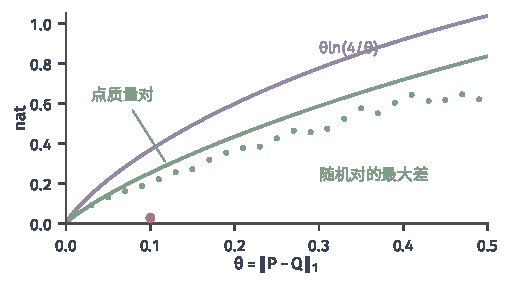
\includegraphics[width=86mm]{figures/07-probability/04-distribution-analysis/matplotlib/info-continuity/figure.pdf}
  \caption{四元字母表上熵差与$\theta=\lVert P-Q\rVert_1$。紫线为界$\theta\ln(4/\theta)$；绿线为点质量$P=(1,0,0,0)$与$Q=(1-\tfrac{\theta}{2},\tfrac{\theta}{6},\tfrac{\theta}{6},\tfrac{\theta}{6})$的熵差；绿点为$200000$对随机分布（种子$1$）在各$\theta$区间内的最大熵差。红点为四字母表与$(0.45,0.3,0.125,0.125)$：$\theta=0.1$，熵差$0.027$。}
  \label{fig:info-continuity}
\end{BookInlineFigure}

图~\ref{fig:info-continuity}比较了界与实际的熵差。离点质量很近的分布熵差最大：把一点质量从确定的结果匀给其余三个值，熵从$0$升到$h_{\mathrm{b}}(\theta/2)+\tfrac{\theta}{2}\ln3$，这条曲线在原点处的斜率同样是无穷大。随机抽取的分布对大多远离这种极端，熵差小得多。四字母表的例子中$\theta=0.1$，界为$0.1\ln40\approx0.369$，实际熵差只有$0.027$：界对最坏情形是合理的，对具体一对分布可能很宽。

\paragraph{有限组合的信息量}
互信息、条件熵在有限字母表上都是几个熵的有限组合，例如$I(X;Y)=H(X)+H(Y)-H(X,Y)$。设$(X,Y)$在$\mathcal{X}\times\mathcal{Y}$上的两个联合分布相差$\theta=\lVert P_{X,Y}-Q_{X,Y}\rVert_1\leq\tfrac12$。边缘分布的$L^{1}$距离不超过联合分布的：
\[
  \sum_x\Bigl\lvert\sum_y\bigl(p(x,y)-q(x,y)\bigr)\Bigr\rvert\leq\sum_{x,y}\lvert p(x,y)-q(x,y)\rvert=\theta.
\]
函数$t\mapsto t\ln(m/t)$在$t\leq m/\mathrm{e}$时递增，所以对边缘也可以用$\theta$代替各自的距离。对三项分别用式~\eqref{eq:info-entropy-continuity}，记$m_X=\lvert\mathcal{X}\rvert$，$m_Y=\lvert\mathcal{Y}\rvert$，得到
\begin{equation}
  \lvert I_P(X;Y)-I_Q(X;Y)\rvert\leq\theta\ln\frac{m_X}{\theta}+\theta\ln\frac{m_Y}{\theta}+\theta\ln\frac{m_Xm_Y}{\theta}.
  \label{eq:info-mi-continuity}
\end{equation}
同样的办法适用于条件熵$H(X\mid Y)=H(X,Y)-H(Y)$和条件互信息。界中的字母表大小来自所用的每一个熵。

\paragraph{无限字母表}
字母表无限时，没有类似的界。取
\[
  P_n=\bigl(1-\tfrac1n\bigr)\delta_0+\tfrac1n\operatorname{Unif}\{1,\dots,K_n\},\qquad K_n=\lceil\mathrm{e}^{n^{2}}\rceil,
\]
它与$\delta_0$的总变差是$\tfrac1n\to0$。设$X\sim P_n$，令$E=\mathbf{1}_{\{X\neq0\}}$。$E$是$X$的函数，由链式法则~\eqref{eq:info-entropy-chain-rule}先揭示$E$再揭示$X$：$E=0$时$X=0$已确定，$E=1$时$X$在$K_n$个值上均匀。于是
\[
  H(P_n)=h_{\mathrm{b}}(\tfrac1n)+\tfrac1n\ln K_n\geq\tfrac1n\cdot n^{2}=n\to\infty,
\]
而$H(\delta_0)=0$。一小份质量被摊到极多的取值上，熵就可以任意大。所以有限字母表上的连续性不能直接推广，需要额外控制质量在远处的分布方式，例如统一的尾部衰减条件。

\paragraph{连续情形与弱收敛}
对密度，弱收敛更不能保证微分熵收敛。在$[0,1]$上取密度
\[
  f_n(x)=1+\sin(2\pi nx),\qquad n=1,2,\dots.
\]
对任意连续函数$\varphi$，$\int_0^1\varphi(x)\sin(2\pi nx)\,\mathrm{d}x\to0$（Riemann–Lebesgue引理），所以$f_n$对应的分布弱收敛于$\operatorname{Unif}(0,1)$，后者的微分熵为$0$。但换元$u=nx$并利用周期性，每个$f_n$的微分熵相同：
\[
  h(f_n)=-\int_0^1(1+\sin2\pi u)\ln(1+\sin2\pi u)\,\mathrm{d}u=\ln2-1\approx-0.307.
\]
振荡越来越快，在任意固定区间上的质量与均匀分布越来越接近，但密度的高低起伏从未减小，微分熵也就停在$\ln2-1$。

\begin{BookInlineFigure}
  \centering
  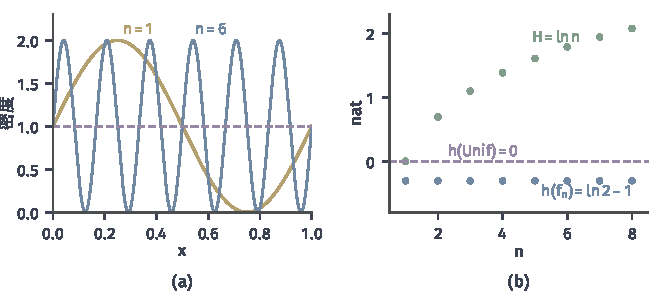
\includegraphics[width=112mm]{figures/07-probability/04-distribution-analysis/matplotlib/info-weak-entropy/figure.pdf}
  \caption{弱收敛不保证熵收敛。(a)密度$f_n(x)=1+\sin(2\pi nx)$，$n=1$（黄）与$n=6$（蓝），紫虚线为极限$\operatorname{Unif}(0,1)$的密度。(b)$h(f_n)$（蓝点，数值积分）恒为$\ln2-1$，极限的微分熵为$0$（紫虚线）；绿点为$\{\tfrac1n,\tfrac2n,\dots,1\}$上均匀分布的熵$\ln n$，它们也弱收敛于$\operatorname{Unif}(0,1)$。单位nat。}
  \label{fig:info-weak-entropy}
\end{BookInlineFigure}

图~\ref{fig:info-weak-entropy}(b)还给出了另一种失效。在$n$个等距点$\tfrac1n,\tfrac2n,\dots,1$上的均匀分布弱收敛于$\operatorname{Unif}(0,1)$，熵是$\ln n\to\infty$，而极限没有概率质量，离散熵无从谈起，只有微分熵$0$。离散分布逼近连续分布时，离散熵按式~\eqref{eq:info-quantized-entropy}的方式发散，要减去$\ln(1/n)$才有有限的极限。

所以在连续空间中谈论信息量的收敛，除了分布本身收敛，还要有关于密度的正则性（如一致有界、等度连续）与尾部的控制。弱收敛只控制有界连续函数的平均，而$-\ln f$既不有界，又随分布本身改变，不在弱收敛能控制的函数之内。


\section{本章小结}
\label{sec:info-summary}

章首问了三件事：一个随机结果平均含有多少不确定性，观测另一个变量能减少多少，以及信息不够时辨别会受到怎样的限制。本章的回答都建立在自信息$-\ln p$上。它由“罕见更意外、独立信息相加”两条要求在相差一个单位常数的意义下唯一确定，以nat或bit计只是刻度不同。

熵是自信息的平均，等于按最佳方式平均要问的是非题数（以bit计，最佳方案与熵相差不到一题）。有限字母表上熵在$0$与$\ln m$之间，两端分别对应确定结果和均匀分布，并且是概率表的凹函数；可数字母表上熵可以为无穷。对密度计算的微分熵可以为负，随坐标伸缩改变$\ln\lvert a\rvert$，它是量化熵减去精度代价$-\ln\Delta$后剩下的部分，二者的极限关系另需正则性与尾部条件。

两个变量时，联合熵不由边缘决定，条件熵是逐条件值的剩余不确定性的平均，链式法则把整体不确定性按揭示顺序分成几段。互信息定义为联合分布相对边缘乘积的KL散度，非负、对称，为零当且仅当独立，可以为无穷，也不要求密度；熵有限时它等于熵之差，由此得到条件化平均不增加熵与联合熵的次可加性。条件互信息衡量已知第三个变量后的共享信息，它与互信息之间没有固定的大小关系。

表~\ref{tab:info-summary}把本章各个量与它们回答的问题、成立条件对照列出。

\begin{BookInlineTable}
  \centering
  \caption{本章的信息量与主要条件}
  \label{tab:info-summary}
  \begin{tabular}{@{}lll@{}}
    \toprule
    量或结论 & 回答的问题 & 需要核对的条件\\
    \midrule
    $H(X)$ & 平均不确定性 & 可数时可能为无穷\\
    $h(X)$ & 密度的平均对数代价 & 可积性；依赖坐标\\
    $H(X\mid Y)$ & 观测后的剩余不确定性 & 只对平均成立\\
    $I(X;Y)$ & 共享信息 & 熵差需各项有限\\
    $H(P,Q)$ & 按参考分布付出的代价 & 零参考概率；$H(P)<\infty$\\
    数据处理 & 后处理不增加信息 & $X\perp\!\!\!\perp Z\mid Y$\\
    Fano & 辨别错误的下界 & 有限标签与猜错标准\\
    InfoNCE & 互信息的可计算下界 & 不超过$\ln N$；总体值\\
    连续性 & 分布接近时信息量接近 & 有限字母表\\
    \bottomrule
  \end{tabular}
\end{BookInlineTable}

交叉熵把平均代价分成固有部分$H(P)$与失配部分$D_{\mathrm{KL}}(P\Vert Q)$；连续时有确定意义的是后者，熵为无穷时也不能用两者之差定义KL。数据处理不等式由互信息链式法则的两种展开得到，前提是处理中的额外随机性在给定观测时与原对象独立；损失恰是条件互信息，可逆变换不损失信息，但不可逆的处理也可能不损失，判据是反向的条件独立。

信息的上界给出辨别的下界：Fano不等式用剩余不确定性限制有限标签的猜错概率，标签均匀时改写为互信息形式，成为通信中超容量不可靠、统计中候选太密无法区分的共同工具。反方向的InfoNCE用辨认真配对的总体损失给出互信息的下界，但下界受候选数$\ln N$与评分函数类的限制，下界小不能推出独立，单批样本值也不自动是下界。最后，有限字母表上熵与互信息对总变差连续，界中含有$\theta\ln(1/\theta)$与字母表大小；无限字母表或连续空间中，接近的分布可以有相差很远的信息量，弱收敛本身不保证熵收敛。

后续各章分别使用这些量。第~\ref{chap:lossless-coding}章到第~\ref{chap:rate-distortion}章研究用熵、互信息衡量的最短描述与有失真描述；第~\ref{chap:discrete-channel-capacity}章到第~\ref{chap:channel-codes}章把容量定义为互信息的最大值，并用Fano不等式证明逆定理；第~\ref{chap:dependence-measures}章把互信息与基于距离、核和离散化的依赖度量放在一起比较。

